\documentclass[12pt]{article}
\usepackage[]{color}
%\usepackage[document]{ragged2e} % for left-aligning, helpful when opening in Word later

%% maxwidth is the original width if it is less than linewidth
%% otherwise use linewidth (to make sure the graphics do not exceed the margin)
\makeatletter
\def\maxwidth{ %
	\ifdim\Gin@nat@width>\linewidth
	\linewidth
	\else
	\Gin@nat@width
	\fi
}
\makeatother

\definecolor{fgcolor}{rgb}{0.345, 0.345, 0.345}
\newcommand{\hlnum}[1]{\textcolor[rgb]{0.686,0.059,0.569}{#1}}%
\newcommand{\hlstr}[1]{\textcolor[rgb]{0.192,0.494,0.8}{#1}}%
\newcommand{\hlcom}[1]{\textcolor[rgb]{0.678,0.584,0.686}{\textit{#1}}}%
\newcommand{\hlopt}[1]{\textcolor[rgb]{0,0,0}{#1}}%
\newcommand{\hlstd}[1]{\textcolor[rgb]{0.345,0.345,0.345}{#1}}%
\newcommand{\hlkwa}[1]{\textcolor[rgb]{0.161,0.373,0.58}{\textbf{#1}}}%
\newcommand{\hlkwb}[1]{\textcolor[rgb]{0.69,0.353,0.396}{#1}}%
\newcommand{\hlkwc}[1]{\textcolor[rgb]{0.333,0.667,0.333}{#1}}%
\newcommand{\hlkwd}[1]{\textcolor[rgb]{0.7te37,0.353,0.396}{\textbf{#1}}}%

%\usepackage{framed}
%\makeatletter
%\newenvironment{kframe}{%
%	\def\at@end@of@kframe{}%
%	\ifinner\ifhmode%
%	\def\at@end@of@kframe{\end{minipage}}%
%\begin{minipage}{\columnwidth}%
%	\fi\fi%
%	\def\FrameCommand##1{\hskip\@totalleftmargin \hskip-\fboxsep
%		\colorbox{shadecolor}{##1}\hskip-\fboxsep
%		% There is no \\@totalrightmargin, so:
%		\hskip-\linewidth \hskip-\@totalleftmargin \hskip\columnwidth}%
%	\MakeFramed {\advance\hsize-\width
%		\@totalleftmargin\z@ \linewidth\hsize
%		\@setminipage}}%
%{\par\unskip\endMakeFramed%
%	\at@end@of@kframe}
%\makeatother

\definecolor{shadecolor}{rgb}{.97, .97, .97}
\definecolor{messagecolor}{rgb}{0, 0, 0}
\definecolor{warningcolor}{rgb}{1, 0, 1}
\definecolor{errorcolor}{rgb}{1, 0, 0}
\newenvironment{knitrout}{}{} % an empty environment to be redefined in TeX

%%% FONT AND INPUT
\usepackage[T5]{fontenc}
\usepackage[utf8]{inputenc} % set input encoding (not needed with XeLaTeX)

%%% Examples of Article customizations
% These packages are optional, depending whether you want the features they provide.
% See the LaTeX Companion or other references for full information.

%%% PAGE DIMENSIONS
\usepackage{geometry} % to change the page dimensions
\geometry{letterpaper} % or letterpaper (US) or a5paper or....
\geometry{margin=1in} % for example, change the margins to 2 inches all round
% \geometry{landscape} % set up the page for landscape
%   read geometry.pdf for detailed page layout information

\usepackage{graphicx} % support the \includegraphics command and options

% \usepackage[parfill]{parskip} % Activate to begin paragraphs with an empty line rather than an indent

%%% PACKAGES
\usepackage{booktabs} % for much better looking tables
\usepackage{array} % for better arrays (eg matrices) in maths
\usepackage{paralist} % very flexible & customisable lists (eg. enumerate/itemize, etc.)
\usepackage{verbatim} % adds environment for commenting out blocks of text & for better verbatim
\usepackage{subcaption} % make it possible to include more than one captioned figure/table in a single float
\usepackage{float}
\usepackage{setspace}
\usepackage{amsmath,newtxtext,newtxmath}
\usepackage{url}
\usepackage{multirow}
\usepackage{listings}
\usepackage{dcolumn}
%\usepackage[nolists]{endfloat}
\usepackage{bbm}
\usepackage{pdflscape}
\usepackage{pdfpages}
\usepackage{xr} % to use \ref with labels from the main text
\externaldocument{'200721 - JOP Draft 2 Appendix'}
\usepackage{tikz} 
\usetikzlibrary{arrows,decorations.pathmorphing,decorations.pathreplacing,backgrounds,fit,positioning,shapes.symbols,chains}

%%% HEADERS & FOOTERS
\usepackage{fancyhdr} % This should be set AFTER setting up the page geometry
\pagestyle{fancy} % options: empty , plain , fancy
\renewcommand{\headrulewidth}{0pt} % customise the layout...
\lhead{}\chead{}\rhead{}
\lfoot{}\cfoot{\thepage}\rfoot{}

%%% CITATION AND BIBLIOGRAPHY

\usepackage[authordate,backend=bibtex8,natbib,sorting=nyt,sortcites,isbn=false,doi=false]{biblatex-chicago}
%\usepackage{natbib}
%\bibliographystyle{apsr}
\bibliography{Literature/library_syp}

% fix problem with \citeyear and \citeyearpar not being highlighted
\DeclareCiteCommand{\citeyear}
	{}
	{\bibhyperref{\printdate}}
	{\multicitedelim}
	{}

\DeclareCiteCommand{\citeyearpar}
	{}
	{\mkbibparens{\bibhyperref{\printdate}}}
	{\multicitedelim}
	{}
% possessive cite with \citepos
\newcommand\citepos[1]{\citeauthor{#1}'s\ (\citeyear{#1})}

% change fnote style to normal text, double-spaced
\renewcommand{\footnotesize}{\normalsize}
\newcommand\fnote[1]{\footnote{\baselineskip=2\normalbaselineskip#1}}
\setlength{\footnotesep}{2pc}

\usepackage{hyperref}
\hypersetup{
	colorlinks=true,
	linkcolor=blue,
	filecolor=magenta,      
	urlcolor=cyan,
}

%%% SECTION TITLE APPEARANCE
\usepackage{sectsty}
%\allsectionsfont{\sffamily\mdseries\upshape} % (See the fntguide.pdf for font help)
% (This matches ConTeXt defaults)

%%% ToC (table of contents) APPEARANCE
\usepackage[nottoc,notlof,notlot]{tocbibind} % Put the bibliography in the ToC
\usepackage[titles,subfigure]{tocloft} % Alter the style of the Table of Contents
\renewcommand{\cftsecfont}{\rmfamily\mdseries\upshape}
\renewcommand{\cftsecpagefont}{\rmfamily\mdseries\upshape} % No bold!

%%% Some commands
\newcommand{\reg}{\texttt{regress} }
\newcommand{\1}{\mathbbm{1}}

\renewcommand\r{\right}
\renewcommand\l{\left}
\newcommand\E{\mathbbm{E}}
\newcommand\V{\mathbbm{V}}
\newcommand\Var{\mathbbm{V}}
\newcommand\avar{{\rm Avar}}
\newcommand\dist{\buildrel\rm d\over\sim}
\newcommand\iid{\stackrel{\rm i.i.d.}{\sim}}
\newcommand\ind{\stackrel{\rm indep.}{\sim}}
\newcommand\cov{{\rm Cov}}
\newcommand{\R}{\textbf{R} }
\newcommand{\Rcmd}[1]{{\large \texttt{#1}}}
\newcommand\indep{\protect\mathpalette{\protect\independenT}{\perp}}
\def\independenT#1#2{\mathrel{\rlap{$#1#2$}\mkern2mu{#1#2}}}
\DeclareMathOperator{\sgn}{sgn}
\DeclareMathOperator*{\argmin}{argmin}

\newcommand\Sum{\sum^N_{i=1}}
\newcommand\Prod{\prod^N_{i=1}}
\newcommand{\pderiv}[1]{\frac{\partial}{\partial #1}}
\newcommand{\B}[1]{\boldsymbol{#1}}
\newcommand{\logit}{\text{logit}}

%%% texcount
% Run texcount on tex-file and write results to a sum-file
\immediate\write18{texcount  \jobname.tex -out=\jobname.sum -incbib -relaxed}
% Define macro \wordcount for including the counts
\newcommand\wordcount{\verbatiminput{\jobname.sum}}

%%%%opening

\title{Tea Leaf Elections: \\
	Inferring Purpose for Authoritarian Elections from Post-election Responses to Defeats%
%	\thanks{I am grateful to Christina Alvarez-Mongote, Julie Bunck, Daniel Hidalgo, Andrew Halterman, Sean Liu, Edmund Malesky, Blair Read, Paul Schuler, Lily Tsai, and participants at MIT Second-Year Paper Workshop and the MPSA Conference 2019, and three anonymous reviewers for their guidance and feedback. Ngoc Phan and Edmund Malesky provided me with the data on Vietnamese government officials.}
	\\
	\vspace{2ex}
	\vphantom{Online Appendix}}
%\author{Minh D. Trinh%
%	\thanks{Doctoral Candidate, Department of Political Science, Massachusetts Institute of Technology. 30 Wadsworth Street E53-415, Cambridge, MA 02142. Phone number: +1-857-600-9241. E-mail: \url{mdtrinh@mit.edu}.}}
\date{July 21, 2020}

\begin{document}
	
%TC:ignore 

\maketitle
\thispagestyle{empty}
\doublespacing

% uncomment this to print title page only
%\end{document}

\begin{abstract}
The power of authoritarian elections is not unlimited. When using elections as a source of information, authoritarian regimes may not be able to collect from a single election all the information it could theoretically provide, and so must judiciously decide which specific signal to seek. It is possible to identify the type of information each regime seeks from its elections by studying its reactions to small but unexpected defeats. Applying this logic to the case of Vietnam, I find that the ruling Communist Party of Vietnam responded to the defeats of its favored candidates in the 2016 election for the national legislature by increasing central transfers to provinces where it suffered these defeats. This evidence suggests that the Party uses elections as an opinion poll to identify areas it is less popular in, instead of as an evaluation device to identify local leaders who under-perform in their electoral mobilization efforts.
\end{abstract}

Word count: 10,490

%TC:endignore 

\newpage

\pagenumbering{arabic}

\section{Introduction}

At first glance, authoritarian elections seem to be an all-powerful weapon in the dictator's arsenal: not only do they rarely pose existential threats, these elections also serve to cement autocrats' rule by providing critical information otherwise unknowable about influential forces both internal and external. The literature that discusses authoritarian elections' many informational functions, however, has not considered potential conflict between them. Autocrats cannot expect authoritarian elections to be informative by default, but must engineer their elections in specific ways to make them informative. However, an election that is designed to provide information on some aspects of governance and social control may become less effective at shedding light on some others. This forces authoritarian rulers to set priorities and use elections as a telescope focused on a few areas of interest, rather than a panoramic camera that captures every information that comes into view.

Without directly observing autocrats' thought processes, how can outside observers identify which, if any, information is being collected through an authoritarian election? In this paper, I propose a framework to identify potentially informative elections, and then to find out which specific informational goals they are serving. Applying this framework to the case of Vietnam, I show that the Communist Party of Vietnam (CPV) needs information on both the sub-national distribution of regime support and on the quality of its local executive officials, but uses elections to learn only about the former. Specifically, I take advantage of rare and unexpected defeats by regime-favored candidates in Vietnam's 2016 legislative election, and use three different empirical methods to show that the CPV increased central transfers to provinces where it has suffered defeats. This finding is consistent with the hypothesis that the regime saw these defeats as indicators for pockets of disillusioned citizens and spent money to placate them. It also rejects the hypothesis that the regime used election defeats to identify provinces with under-performing local officials. Under this alternative hypothesis the CPV would have wanted to punish officials in these provinces, but the increased central transfers would have accomplished only the opposite.

Using empirical evidence from the case of Vietnam, this paper contributes to the larger literature on authoritarian elections. Its main theoretical contribution is to demonstrate how existing theories about authoritarian elections' functions may contradict each other when applied to some certain cases -- specifically those that portray elections as the autocrat's opinion poll \citep[e.g.][]{Miller2015, Magaloni2006, Blaydes2010} and those that portray them as a test to evaluate regime agents \citep[e.g.][]{Magaloni2006, Blaydes2010,Myagkov2009,RundlettSvolik2016}. In addition, it offers a framework to identify autocrats' motivations and test theories of authoritarian elections using post-election responses to localized defeats. Finally, the finding suggests that even rulers of stable authoritarian regimes like Vietnam may still respond to public dissatisfaction, suggesting possible pathways for accountability through formal authoritarian institutions.

\section{Making Authoritarian Elections Informative}
\label{sec:lit_review}

Why do some authoritarian regimes choose to hold elections, and then allow less-than-satisfactory results to happen, when they could have gotten away without them? The literature on authoritarian elections has proposed that elections may bring enough benefits for autocrats to justify their potential risks.\fnote{See \citet{LustOkar2005, AR2005, Magaloni2006, Blaydes2010, Miller2015, Cox2009, Geddes2018} for some seminal works.} Most commonly, this literature shows that authoritarian elections provide autocrats with different types of information, such as about their opponents' strength \citep[][Ch. 6]{Geddes2018}, the existence of potential threats or allies \citep{LustOkar2005}, the competence or loyalty of their agents \citep{Magaloni2006, Blaydes2010, Myagkov2009, RundlettSvolik2016}, the citizenry's \textit{level} of dissatisfaction with the regime \citep{Miller2015} or even its \textit{distribution} across sub-national units \citep{Magaloni2006, Blaydes2010}. All this information then contributes to authoritarian longevity by allowing the regime to adjust its policies, either by suppressing opposition strongholds \citep{Magaloni2006, Blaydes2010} buying off dissatisfied public \citep{Miller2015, Magaloni2006}, or co-opting emerging elites into the regime \citep{LustOkar2005}.

Other scholars \citep[e.g.][]{Rozenas2016,Wintrobe2000, Morgenbesser2016}, however, argue that good information does not emerge easily out of authoritarian elections. They note an important trade-off between authoritarian elections' primary functions: when autocrats use manipulation to win elections, they end up lowering their information value. Indeed, the more uncertainty manipulation tactics remove from an election, the less variation remains in the results to shed light on any internal or external forces that could have otherwise manifested in the vote counts.

Information collection through authoritarian elections is further challenged by the complexity of the information being generated. Specifically, when there are multiple potential ways to interpret a particular set of results, regime leaders may not be able to draw solid conclusions from the raw numbers that make up an election's outcome. For example, a humiliating setback in an electoral district, the regime must determine whether the cause behind it is unenthusiastic regime agents not manipulating the election well enough, or disenchanted citizens frustrated enough to risk voting against the ruling party. Depending on how the regime interprets the defeat, it would learn something either about the quality of its agents or about the distribution of its popularity across the country. If both interpretations are equally plausible the regime would find it hard to decide which interpretation to commit to; even when it chooses to believe in both -- as a ``weighted mixture'' for instance -- there can be an infinite numbers of differently weighted mixtures that could explain equally well the observed results.

When and how, then, can authoritarian elections provide useful information? These elections may become informative when authoritarian regimes engage in \textit{selective manipulation}: by combining careful restraint in some domains with bold manipulation in others, they may allow some informative variation in the results, yet still reduce both electoral risks and informational complexity. Restraint is necessary because an election's results can only be informative of any societal force if it is allowed to influence the vote tallies. At the same time, to know for sure that the results they observe are truly informative of the one variable they care about, autocrats also need manipulation tactics that prevent others from entering the equation. In this sense, strategies that place rigid controls on some moving parts of the electoral process not only win elections, but also help reduce the complexity of the information that these elections may generate. By heavily engaging in these strategies while exercising relative restraint in others, authoritarian leaders can decide which sources of electoral variation to shut down and which sources to draw information from, thereby achieving both security and information. This selective manipulation logic offers another explanation for why many authoritarian regimes use only a subset of manipulation tactics available to them e.g. Singapore's government tilting electoral rules in favor of the ruling party but refrains from vote fraud \citep{Tan2013}, or China's banning all opposition parties but allow individual independents \citep[see][]{Junzhi2010}.

Selective manipulation, however, is only attainable by some authoritarian regimes. First, they must be secure enough to not require unrestrained manipulation on all fronts, or to tolerate limited risks without feeling existentially threatened. Second, the regime's leaders must exercise a high degree of control over its agents through a disciplined party apparatus, so as to oversee which manipulation strategies are and are \textit{not} being carried out. It is thus no surprise that existing literature have mostly documented information collection through authoritarian elections in relatively secure hegemonic, dominant-party or one-party regimes where elections are rarely competitive, such as Mexico \citep{Magaloni2006}, Egypt \citep{Blaydes2010}, Jordan \citep{LustOkar2005}, Russia \citep{Myagkov2009, RundlettSvolik2016}, Malaysia \citep{Brownlee2007} or Singapore \citep{Miller2015}. In practice, other constraints or even mistakes may lead autocrats to misjudge the fine balance between manipulation and restraint. Furthermore, because autocrats may avoid some manipulation tactics for other strategic reasons, evidence of selective manipulation strongly suggests but still does not confirm that they have an informational interest in authoritarian elections.

\section{The Informational Limits of Authoritarian Elections}
\label{sec:theory_limits}

The informational value of authoritarian elections are limited in yet another way: even when it is engineered to be informative, no single election can provide every piece of information that authoritarian elections are said to provide. Indeed, an election designed to be a jack of all trades only risks becoming a master of none: the more types of information a dictator seeks from an election, the less effective it becomes at acquiring any of them. There are several reasons for this:

Firstly, for authoritarian elections to be informative, autocrats need to reduce their informational complexity with selective manipulation. Selective manipulation works best if it completely shuts down undesirable determinants of election outcomes, yet when it does no information can be learned about these determinants. In other words, tactics to ensure elections send clear signals about some types of information also prevent them from sending any signal about others.

Secondly, selective manipulation also means selective restraint, which even when attainable may still compromise other non-informational objectives of authoritarian elections. Even if authoritarian regimes who collect information with selective manipulation do not worry about losing, many of them may have other goals for their elections, some of which may be jeopardized even by a minimal extent of restraint. For example, even as some authoritarian regimes seek legitimation by tolerating or even inviting some apparent electoral setbacks, others build their legitimacy on the foundation of large or absolute victories (\citet{Morgenbesser2016, Simpser2013, Geddes2018}). Their need for overwhelming margins limits the effective tolerance for selective restraint, which then prevents them from collecting as much information as they could from elections.

Most importantly, a regime seeking to infer different types of information from the same election may face difficulty in making policy adjustments in reaction to all the incoming information. Moreover, the suitable response to one information may end up contradicting the response to another: a regime perceiving election setbacks as information about incompetent regime agents may choose to punish them, but in doing so it may embolden disobedient citizens by helping them get rid of incongruent officials. The potential for such conflict in post-election responses is especially serious for regimes whose repertoire of actions is limited, as in the case of low-capacity regimes, but also high-capacity regimes with highly structured institutions and low level of policy discretion. For these regimes, seeking too much information from elections only results in contradictory policy recommendations, which debilitates more than facilitates policy responsiveness. The solution, then, is to design their elections to provide only the kind of information they can coherently react to. If this is not possible, autocrats must willfully ignore some plausible information and pay attention to only what they need to know, accepting the possibility of learning the wrong lesson entirely. 

\subsection{Informational Limits of Vietnam's National Assembly Elections}
\label{sec:vietnam_limits}
Vietnam exemplifies an authoritarian regime that needs and thus seeks information from elections, but faces a limit in how many different types of information it can get from one election. It is a single-party regime, which formally follows a parliamentary system but in practice is centrally ruled by the Communist Party of Vietnam (CPV). Like most authoritarian regimes, the CPV needs a reliable flow of information from the citizenry and regime agents. Thanks to a large and deeply penetrating security apparatus, it has managed to secure much of this information \citep[see][]{Thayer2014}. It does not, however, have sufficient information on two variables: the distribution of regime support across sub-national units, and the quality of its subordinates at local levels of government. 

In terms of public support, the Vietnamese regime only has reasons to feel confident about its general \textit{level} of popularity: the CPV benefits from a historical legacy as the revolutionary party that brought independence from the French in 1945 and unified the country in 1975, from the recent period of economic growth, as well as from its tight control over the media and other propaganda apparatus. Indeed, even international surveys such as the World Values Survey \citeyearpar{wvs} and the Asian Barometer Survey have consistently found very high levels of trust in the government. At the same time, the government in Hanoi cannot be confident that its popularity is evenly \textit{distributed} among the population of more than 90 million and across a territory spanning more than 15 degrees latitude. Although protests or riots are rare, unrest has occasionally emerged from isolated pockets of dissatisfaction, such as in Binh Thuan in 2018, Hanoi in 2017, or Ha Tinh in 2016. 

The CPV, however, has few reliable instrument to detect potential protests before they emerge. Not only are international surveys covering too few respondents to provide reliable sub-national estimates, the regime's own attempts at studying public opinion are also inadequate.\fnote{In a personal interview, an official in the CPV's public opinion research unit claims that it conducts 9 to 10 surveys a year, but admits that they are not large-scale surveys that can be quantitatively analyzed. Instead, it relies primarily on networks of grassroot informants whose reports do not allow for effective cross-region comparison.} %\fnote{Personal interview with an official in the CPV's public opinion research unit, Hanoi 2018.}
In addition, other information sources also prove insufficient: the media is largely muted, whereas reporting by local government officials are likely subjected to intentional embellishment, because these officials are evaluated for promotion based on their ability to maintain low levels of dissent.

In terms of regime agents, the CPV needs unbiased and standardized information about its millions of government and party bureaucrats. For the CPV, the quality of local bureaucrats matters through its effect on the party's popularity among the populace, but for personnel management reasons as well. Vietnam has a cadre management system which provides regime subordinates with meritocratic promotion pathways in exchange for their loyalty \citep{Svolik2012}, but requires that the party can discern bureaucrats' true ability to function properly. In addition, because the central leadership in Hanoi delegates significant power to the periphery, particularly at the province level, it needs information to determine the loyalty of provincial executive officials.\fnote{Each provincial government typically has two executives, the Secretary of the Party Committee who represent the Party and the Chairman of the People's Councils who represent the Government. The Party Secretary is considered as the superior position.} Not only do disloyal executives pose challenges to the regime's authority, because some of them may one day be promoted to the highest tier of the party leadership, knowing where their ultimate loyalty lies is critical for the CPV's future. This concern is particularly relevant because nearly two thirds of these officials serve in their home provinces and have strong local ties that may supersede Hanoi's authority. %\fnote{According to data from \citet{MaleskyPhan2017}.}
Even for outsiders directly appointed by Hanoi, local interests still exert significant influence, particularly through the rank-and-file bureaucrats who are almost always natives.

The Vietnamese regime already possesses instruments to collect a large amount of information on their agents, but their reliability and neutrality is questionable. On one hand, the primarily outcome- and output-based measures that make up official reporting channels do not account for variation in external factors, rendering achievements inherently incomparable across sub-national units. On the other hand, because the collection and compilation of performance measures is such a massive endeavor, the CPV has to delegate the majority of the work to sub-national officials. This gives these officials both the incentive and the capacity to misreport the indicators they are evaluated on \citep[][Ch. 8]{JensenMalesky2018}.

\subsection{VNA Elections as Plausible Information Gathering Tools}

At first glance, the VNA elections have important non-informational goals to fulfill. Occurring every four to five years, these elections would fill the approximately 500 seats in the country's national legislature from a pool of roughly 800 candidates. Nearly a quarter of these candidates are minister-level officials in central-level party or government institutions, current VNA subcommittee members, or national leaders of state-sanctioned mass organizations. Prior to the election day these central candidates are allocated to local-level electoral districts, where they run alongside local candidates who are often province-level officials or elites. The CPV strongly prefers central candidates to win. Symbolically, central candidates are key party elites for whom defeat would be embarrassing. Practically, many of these candidates are pre-designated to hold high-level positions in both the VNA and in the central government, for which membership in the VNA is required.\fnote{Some observers suspect that the regime may want some of these candidates to lose, for example to project the image of truly competitive elections \citep{Morgenbesser2016}. The CPV, however, has never tied its legitimacy to claims about electoral competitiveness in official narratives. Citizens themselves overwhelmingly stated that they do not believe elections to be even remotely competitive (personal interviews, Hanoi and Ho Chi Minh City, 2016-2017).}

Additionally, before each election, the central leadership also draws up a structure of what the next legislature should look like, down to specific quotas along demographic, political and functional lines \citep{MaleskySchuler2009}. The CPV then uses the tools at its disposal to ensure that the elected candidates together form a legislature as close to the planned structure as possible.

Even with these non-informational objectives, the Vietnamese regime does seem to use elections for some additional informational goals. A telling evidence is that the CPV does not utilize every possible manipulation tactic available to them, accepting instead to keep certain dimensions of the elections imperfectly regulated. Particularly, the CPV relies mostly on electioneering and mass mobilization, both of which occurs prior to the election day, rather than heavy-handed tactics such as vote-buying or ballot stuffing \citep{MaleskySchuler2011}.\fnote{See evidence from digit tests in \citet{MaleskySchuler2011} and in Online Appendix \ref{app:benford} (2-4)}

The CPV's electioneering efforts rely primarily on its control of candidate lists in electoral districts. Firstly, it filters out most independent and self-nominated candidates who are deemed to pose serious threats. Secondly, it allocates most central candidates to districts with particularly favorable candidate-to-seat ratios.\fnote{Depending on population size, each district can have 4, 5 or 6 candidates, and is allowed 2, 3, or 4 VNA seats. Each voter votes for as many candidates as there are seats. The candidates with the most votes win as long as their vote shares exceed 50 percent. Central candidates could lose if too many of the local candidates win too much of the vote share, or if they themselves fail to secure approval from at least half of the voters. Either outcome is less likely in districts with 5 candidates, as their seat-to-candidates ratio of $0.6$ is more favorable than in other districts.} Thirdly, within these districts, central candidates face only local candidates with weaker profiles, and typically do not have to run against and split votes with other central candidates. Finally, the party bunches candidates with similar profiles together in each district, e.g. by making all under-40 women run against each other, such that no matter which candidate wins the district's winner still fits the same profile quota. As a result, even when individual candidates may compete against each other, central candidates normally come out on top, and the aggregate structure of the VNA is also guaranteed \citep{MaleskySchuler2011}. 

In addition to electioneering, the CPV also conducts a massive mobilization campaign prior to and even on election day. As part of this campaign, cadres at the neighborhood or village level visit individual households to educate voters about the election process. During these visits, the cadres would give explicit ``suggestions'' about which candidates to vote for.\fnote{Personal observations, Ha Noi, 2011; Personal interviews, Ha Noi and Ho Chi Minh City, 2016-2017} On election day, the same cadres would visit the households again to convince people to go vote, and even carry mobile ballot boxes to those unable to come to the polling station themselves.

These strategies are able to deliver election results very close to what the regime expects: in all the recent elections, the structure of the elected VNA has always been nearly identical to what Hanoi plans,\fnote{See Table 1 in \citet[][506]{MaleskySchuler2011} for details} and most central candidates end up getting elected, usually with large margins and near-universal turnout across the country.\fnote{Proxy voting, usually in the form of one person voting for the entire household, is common.} At the same time, these results are not perfect. Most importantly, a small number of central candidates -- 21 out of 165 for 2007, 14 out of 173 for 2011, and 16 out of 197 for 2016 -- lose elections, and their defeats were surprising and disappointing enough that even the state-controlled media has covered them \citep[e.g.][]{vov2016}. Certainly, a degree of electoral risk still exists in Vietnam's tightly managed elections.%\fnote{\citet[][106-107]{Schedler2013} distinguishes between hegemonic and competitive autocracies by the level of uncertainty faced by the ruling party. Despite the uncertainty over the central candidates' performance, Vietnam should still be considered a hegemonic regime, as this uncertainty has only limited impact over the regime's control over society.}

Given the CPV's yet unsolved information deficit, it seems plausible that it also uses the VNA elections for informational goals. National election results offer superior information for many reasons: they are collected across the country and tabulated at every administrative level, are measured in standardized metrics, and are overseen by both central-level and local-level officials.

Consistent with the profile of an authoritarian regime intentionally tolerating electoral risk in exchange for information, the CPV evidently engages in selective manipulation. First, some of their strategies could be seen as attempts to refine the range of plausible interpretations for the incoming results. For example, because most central candidates do not get assigned to provinces they have served in or even to their home provinces, the results reflect neither their past performance nor their individual popularity. Similarly, because most high-profile dissidents have been banned, the final tallies would not reflect voters' empathy for any particular regime opponents.

More importantly, CPV leaders refrain from some of the most direct forms of manipulation even when they could afford them. Indeed, the variables Hanoi selectively allows to influence election outcomes correspond exactly to its two most pressing informational needs -- the local level of regime popularity and the quality of local officials. First, the choices on the ballots all but enable voters to channel their opinion of the regime through their votes for central candidates. Because these candidates are mostly strangers to their constituencies, the cadres' instructions give voters plenty of cues to associate them with the central party leadership. With no other context about their performance, voters have only this association to inform their vote. At the same time, the anonymity afforded by the near-universal turnout and the seemingly secret ballot encourages voters to express dissatisfaction without fear of retribution.\fnote{Voters' confidence in their anonymity ironically stems from a distrust of the tabulation of results: they think that ballots are not traceable to individuals because the regime would not even look at them, choosing instead to make up results when tabulating vote counts. Personal interviews, Ha Noi and Ho Chi Minh City, 2016-2017.}\fnote{Experts who evaluated the most recent VNA election for the Perception of Electoral Integrity dataset \citep{PEI} believed that ballot boxes are not completely confidential, but rated the extent of this problem much lower (at 3 out of 5 points) compared to most other forms of violation such as biased election laws (5), blocking of opposition candidates (4.88), or unequal access to the media (4.57).} Central candidates become clear targets for such disapproval: among voters who willingly expressed dissatisfaction with the regime, many claimed that they crossed out the very candidate local cadres had instructed them to support.\fnote{Personal interviews, Ha Noi and Ho Chi Minh City, 2016-2017}

In regard to province-level officials, the CPV allows their competence and loyalty to factor in election outcomes even when clear center-periphery conflict of interests could arise. Specifically, although central party leaders decide on demographic quotas for the incoming VNA and nominate central candidates, they delegate most electioneering and mobilization efforts to provincial executives, including the discretion over candidate lists and the logistics of mobilization campaigns. Provincial officials find it in their interest to use this power to support central candidates, but not so eagerly that local candidates are hurt. Indeed, each elected central candidate takes away one VNA seat from local candidates; this creates enough tension that the municipality of Hanoi even demanded to receive fewer central candidates in 2016 \citep{vnexpress2016_2}. Furthermore, central candidates who win by large margins may make some local candidates fail the 50 percent threshold, costing the province seats that are otherwise secure. Because many top provincial officials also run as local candidates, and because VNA seats give provinces representation in the legislature, provinces need to balance their support between central and local candidates. Central candidates may lose if provincial officials unintentionally miscalculate or intentionally disregard this balance.

The CPV's inferential problem arises from the fact that any information to be gained about regime popularity and regime agents quality at the province level are both tied to the electoral performance of central candidates allocated to each province. In other words, these candidates' performance can tell the regime two different but observationally equivalent stories: bad results either suggest areas where the CPV is unpopular, or identify provincial executives who fail or have shirked their duties. \textit{A priori}, both stories are plausible given the CPV's selected manipulation tactics, but there is no indication which of them it is more inclined to believe in.

\section{Responses to Localized Defeats Reveal Purpose(s) of Authoritarian Elections}
\label{sec:theory_local_defeat}

Observing authoritarian regimes like Vietnam’s selectively pursuing some manipulation strategies while refraining from others may give outsiders reasons to suspect them of using elections as an information source, but this is hardly a smoking gun. Some autocrats may avoid some forms of malfeasance for other strategic reasons, and others may erroneously exercise restraint where they have no informational need to do so. Furthermore, even when a regime exercises multiple forms of restraint as if they are seeking multiple types of information, the argument in Section \ref{sec:theory_limits} suggests that they would not pursue all of them at once. How can outsiders know for sure which specific information, if any, is being sought from these elections, short of asking the dictators themselves?  I propose the following approach: observe their \textit{a posteriori} reaction to some signal from elections, preferably when such signal is so clear that a reaction has to be expected, and then use backward induction to determine what kind of information the dictator had received from the signal. \textit{Localized defeats} -- defeats of regime candidates in local constituencies, despite the regime's manipulation in their favor -- provide one such opportunity.

%There are many reasons localized defeats can happen under authoritarian regimes, as they had in Singapore \citep{Ortmann2011, Miller2015}, Russia \citep{Gelman2013}, or particularly Vietnam \citep{MaleskySchuler2011}. They are particularly likely in parliamentary elections, when a relatively large number of regime candidates run in a relatively large number of constituencies, creating many opportunities for any of them to fail. Defeats of regime candidates often result from effective strategies by the opposition \citep{BunceWolchik2010} or certain regime weaknesses \citep{LevistkyWay2010}, but even under strong authoritarian regimes they are possible. Most particularly, when dictators seek information from elections they may intentionally loosen up their control over certain aspects of the electoral process, allowing the opposition an opening.

Localized defeats can and did happen under many secure authoritarian regimes, as they had in Singapore \citep{Ortmann2011, Miller2015}, Russia \citep{Gelman2013}, or particularly Vietnam \citep{MaleskySchuler2011}. They are likely in parliamentary elections, when many regime candidates run in many constituencies, but also happen in presidential systems, in the form of districts that do not go to the incumbent. Localized defeats are a good lens into an authoritarian regime's informational needs because they are high-information events. Since authoritarian regimes rarely suffer and thus do not expect unsatisfactory results, any defeat would provide a data point so different from their informational prior, guaranteeing that it contains more signal than noise. Indeed, even when variation in vote shares is a function of both signal and noise, a defeat indicates an alarmingly low vote share that could only result from a true aberration on the ground. Thus, if a regime is truly using elections as a source of information, it should always pay attention to localized defeats. 

If the regime acknowledges the information from localized defeats, it should also respond with some actions -- after all, what good is \textit{information} if it does not \textit{inform} any action? At the minimum, as long as autocrats prefer winning over losing they would have some response to the defeats, even if only to avoid their repetition. Indeed, given that most existing informational theories of authoritarian elections rest on the exact premise that regime leaders collect information from elections to calibrate their actions, these theories would also predict that they make behavioral change following the high dose of information from localized defeats. 

\begin{figure}[H]

\centering
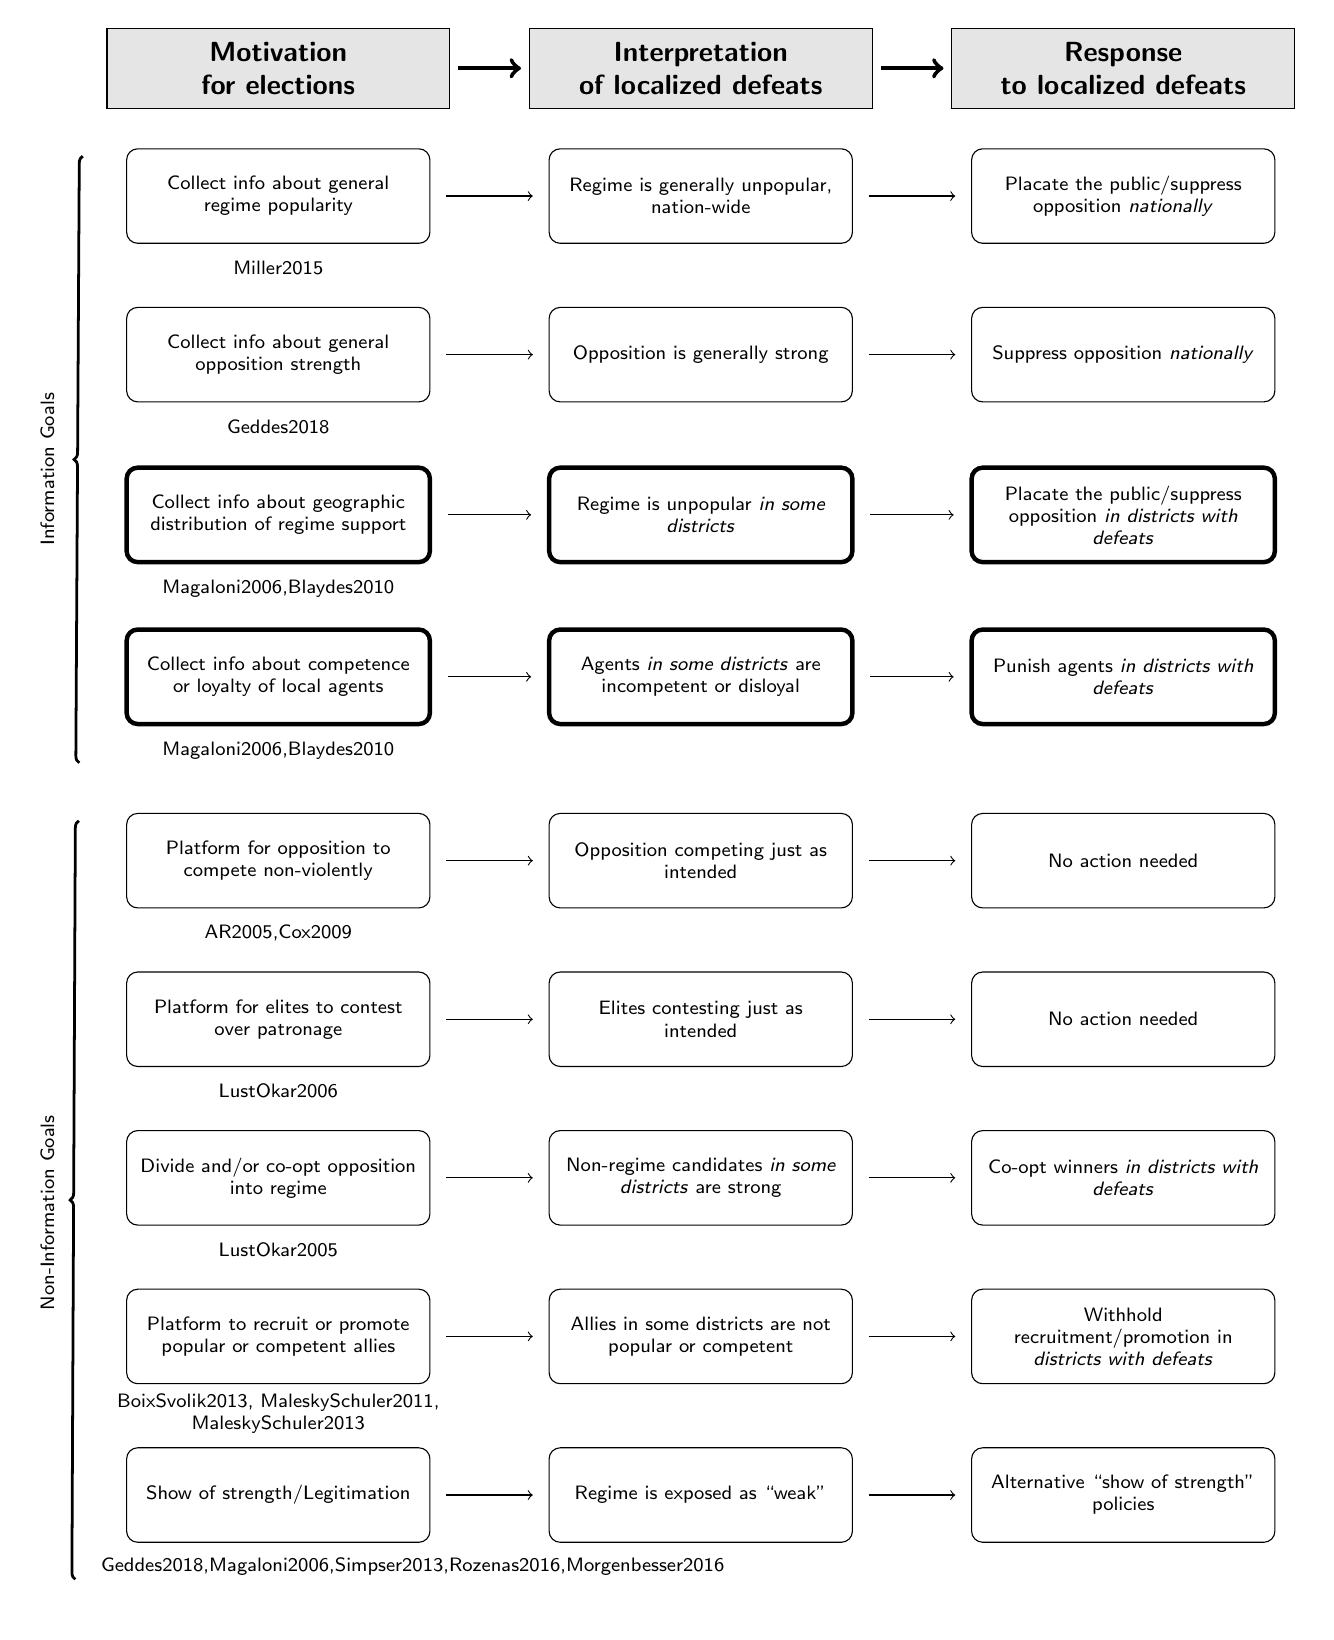
\begin{tikzpicture}
[node distance = 1cm, auto,font=\footnotesize,
% STYLES
every node/.style={node distance=3cm},
% The title style is used to draw the main title
title/.style={rectangle, draw, fill=black!10, inner sep=5pt, text width=4cm, text badly centered, minimum height=1cm, font=\bfseries\footnotesize\sffamily},
% The subtitle style is used to draw the title below main title
subtitle/.style={rectangle, inner sep= 2pt, minimum height=.5cm, node distance=0.25cm, text width=4.5cm, text badly centered, font=\scriptsize\sffamily},
% The theory style is used to draw nodes for each theory
theory/.style={rectangle, rounded corners, draw, minimum height=1.2cm, inner sep= 5pt, text width=3.5cm, node distance=0.25cm, text badly centered, font=\scriptsize\sffamily}]

%%%% Top nodes %%%%
\node [title] (interpretation) {Interpretation\\of localized defeats};
\node [title, left=1cm of interpretation] (intention) {Motivation\\for elections};
\node [title, right=1cm of interpretation] (response) {Response\\to localized defeats};

%% Top nodes subtitle

% Intention
%\node [subtitle, below=0.2cm of intention] (sub-intention) {for\\
%	authoritarian elections};

% Interpretation
%\node [subtitle, below=0.2cm of interpretation] (sub-interpretation) {of\\
%	localized defeats};

% Response
%\node [subtitle, below=0.2cm of response] (sub-response) {to\\
%	localized defeats};

%%%% Theory nodes %%%%
% B1
\node [theory, below=0.5cm of intention] (B1-intention) {Collect info about general regime popularity};
\node [subtitle, below=0.05cm of B1-intention] (B1-sub-intention) {\citep{Miller2015}};

\node [theory, below=0.5cm of interpretation] (B1-interpretation) {Regime is generally unpopular, nation-wide};
\node [subtitle, below=0.05cm of B1-interpretation] (B1-sub-interpretation) {};

\node [theory, below=0.5cm of response] (B1-response) {Placate the public/suppress opposition \textsl{nationally}};
\node [subtitle, below=0.05cm of B1-response] (B1-sub-response) {};

% B2
\node [theory, below=0.8cm of B1-intention] (B2-intention) {Collect info about general opposition strength};
\node [subtitle, below=0.05cm of B2-intention] (B2-sub-intention) {\citep{Geddes2018}};

\node [theory, below=0.8cm of B1-interpretation] (B2-interpretation) {Opposition is generally strong};
\node [subtitle, below=0.05cm of B2-interpretation] (B2-sub-interpretation) {};

\node [theory, below=0.8cm of B1-response] (B2-response) {Suppress opposition \textsl{nationally}};
\node [subtitle, below=0.05cm of B2-response] (B2-sub-response) {};

% B3
\node [theory, below=0.8cm of B2-intention, ultra thick] (B3-intention) {Collect info about geographic distribution of regime support};
\node [subtitle, below=0.05cm of B3-intention] (B3-sub-intention) {\citep{Magaloni2006,Blaydes2010}};

\node [theory, below=0.8cm of B2-interpretation, ultra thick] (B3-interpretation) {Regime is unpopular \textsl{in some districts}};
\node [subtitle, below=0.05cm of B3-interpretation] (B3-sub-interpretation) {};

\node [theory, below=0.8cm of B2-response, ultra thick] (B3-response) {Placate the public/suppress opposition \textsl{in districts with defeats}};
\node [subtitle, below=0.05cm of B3-response] (B3-sub-response) {};

% B4
\node [theory, below=0.8cm of B3-intention, ultra thick] (B4-intention) {Collect info about competence or loyalty of local agents};
\node [subtitle, below=0.05cm of B4-intention] (B4-sub-intention) {\citep{Magaloni2006,Blaydes2010}};

\node [theory, below=0.8cm of B3-interpretation, ultra thick] (B4-interpretation) {Agents \textsl{in some districts} are incompetent or disloyal};
\node [subtitle, below=0.05cm of B4-interpretation] (B4-sub-interpretation) {};

\node [theory, below=0.8cm of B3-response, ultra thick] (B4-response) {Punish agents \textsl{in districts with defeats}};
\node [subtitle, below=0.05cm of B4-response] (B4-sub-response) {};

% A1
\node [theory, below=1.1cm of B4-intention] (A1-intention) {Platform for opposition to compete non-violently};
\node [subtitle, below=0.05cm of A1-intention] (A1-sub-intention) {\citep{AR2005,Cox2009}};

\node [theory, below=1.1cm of B4-interpretation] (A1-interpretation) {Opposition competing just as intended};
\node [subtitle, below=0.05cm of A1-interpretation] (A1-sub-interpretation) {};

\node [theory, below=1.1cm of B4-response] (A1-response) {No action needed};
\node [subtitle, below=0.05cm of A1-response] (A1-sub-response) {};

% A2
\node [theory, below=0.8cm of A1-intention] (A2-intention) {Platform for elites to contest over patronage};
\node [subtitle, below=0.05cm of A2-intention] (A2-sub-intention) {\citep{LustOkar2006}};

\node [theory, below=0.8cm of A1-interpretation] (A2-interpretation) {Elites contesting just as intended};
\node [subtitle, below=0.05cm of A2-interpretation] (A2-sub-interpretation) {};

\node [theory, below=0.8cm of A1-response] (A2-response) {No action needed};
\node [subtitle, below=0.05cm of A2-response] (A2-sub-response) {};

% C1
\node [theory, below=0.8cm of A2-intention] (C1-intention) {Divide and/or co-opt opposition into regime};
\node [subtitle, below=0.05cm of C1-intention] (C1-sub-intention) {\citep{LustOkar2005}};

\node [theory, below=0.8cm of A2-interpretation] (C1-interpretation) {Non-regime candidates \textsl{in some districts} are strong};
\node [subtitle, below=0.05cm of C1-interpretation] (C1-sub-interpretation) {};

\node [theory, below=0.8cm of A2-response] (C1-response) {Co-opt winners \textsl{in districts with defeats}};
\node [subtitle, below=0.05cm of C1-response] (C1-sub-response) {};

% C2
\node [theory, below=0.8cm of C1-intention] (C2-intention) {Platform to recruit or promote popular or competent allies};
\node [subtitle, below=0.05cm of C2-intention] (C2-sub-intention) {\citep{BoixSvolik2013, MaleskySchuler2011, MaleskySchuler2013}};

\node [theory, below=0.8cm of C1-interpretation] (C2-interpretation) {Allies in some districts are not popular or competent};
\node [subtitle, below=0.05cm of C2-interpretation] (C2-sub-interpretation) {};

\node [theory, below=0.8cm of C1-response] (C2-response) {Withhold recruitment/promotion in \textit{districts with defeats}};
\node [subtitle, below=0.05cm of C2-response] (C2-sub-response) {};

% D1
\node [theory, below=0.8cm of C2-intention] (D1-intention) {Show of strength/Legitimation};
\node [subtitle, below=0.05cm of D1-intention] (D1-sub-intention) {\citep{Geddes2018,Magaloni2006,Simpser2013,Rozenas2016,Morgenbesser2016}};

\node [theory, below=0.8cm of C2-interpretation] (D1-interpretation) {Regime is exposed as ``weak''};
\node [subtitle, below=0.05cm of D1-interpretation] (D1-sub-interpretation) {};

\node [theory, below=0.8cm of C2-response] (D1-response) {Alternative ``show of strength'' policies};
\node [subtitle, below=0.05cm of D1-response] (D1-sub-response) {};

%%%% Side theory category nodes %%%%

% B
\node [subtitle, left=1cm of B1-intention.north west, rotate=90, text width = 8cm] (information) {Information Goals};

\draw [decorate,decoration=brace, line width=1pt] 
([xshift=-0.2cm, yshift=0.1cm]B4-sub-intention.south west) -- ([xshift=-0.55cm, yshift=-0.1cm]B1-intention.north west);

% A, C and D together
\node [subtitle, left=1cm of A1-intention.north west, rotate=90, text width = 10cm] (non-information) {Non-Information Goals};

\draw [decorate,decoration=brace, line width=1pt] 
([xshift=-0.25cm, yshift=0.1cm]D1-sub-intention.south west) -- ([xshift=-0.6cm, yshift=-0.1cm]A1-intention.north west);

%% A
%\node [subtitle, left=0.6cm of A1-intention.north west, rotate=90, text width = 4.4cm] (power-sharing) {``Platform''/``Power-sharing''};
%
%\draw [decorate,decoration=brace, line width=1pt] 
%([xshift=-0.2cm, yshift=0.1cm]A2-sub-intention.south west) -- ([xshift=-0.2cm, yshift=-0.1cm]A1-intention.north west);
%
%% C
%\node [subtitle, left=0.6cm of C1-intention.north west, rotate=90, text width = 1.9cm] (co-optation) {``Co-optation''};
%
%\draw [decorate,decoration=brace, line width=1pt] 
%([xshift=-0.2cm, yshift=0.1cm]C2-sub-intention.south west) -- ([xshift=-0.2cm, yshift=-0.1cm]C1-intention.north west);
%
%% D
%\node [subtitle, left=0.6cm of D1-intention.north west, rotate=90, text width = 2cm] (show-of-strength) {``Demonstration''};
%
%\draw [decorate,decoration=brace, line width=1pt] 
%([xshift=-0.2cm, yshift=0.1cm]D1-sub-intention.south west) -- ([xshift=-0.2cm, yshift=-0.1cm]D1-intention.north west);


%%%%%%%%%%%%%%%%

% Draw the links between forces
\path[->,ultra thick, shorten >=.1cm, shorten <=.1cm] 
(intention) edge (interpretation)
(interpretation) edge (response);

\path[->, shorten >=.2cm, shorten <=.2cm] 
(A1-intention) edge (A1-interpretation)
(A1-interpretation) edge (A1-response);

\path[->, shorten >=.2cm, shorten <=.2cm] 
(A2-intention) edge (A2-interpretation)
(A2-interpretation) edge (A2-response);

\path[->, shorten >=.2cm, shorten <=.2cm] 
(B1-intention) edge (B1-interpretation)
(B1-interpretation) edge (B1-response);

\path[->, shorten >=.2cm, shorten <=.2cm] 
(B2-intention) edge (B2-interpretation)
(B2-interpretation) edge (B2-response);

\path[->, shorten >=.2cm, shorten <=.2cm] 
(B3-intention) edge (B3-interpretation)
(B3-interpretation) edge (B3-response);

\path[->, shorten >=.2cm, shorten <=.2cm] 
(B4-intention) edge (B4-interpretation)
(B4-interpretation) edge (B4-response);

\path[->, shorten >=.2cm, shorten <=.2cm] 
(C1-intention) edge (C1-interpretation)
(C1-interpretation) edge (C1-response);

\path[->, shorten >=.2cm, shorten <=.2cm] 
(C2-intention) edge (C2-interpretation)
(C2-interpretation) edge (C2-response);

\path[->, shorten >=.2cm, shorten <=.2cm] 
(D1-intention) edge (D1-interpretation)
(D1-interpretation) edge (D1-response);


\end{tikzpicture} 
\caption{Key theories of authoritarian elections and their predictions about how regime leaders perceive and respond to localized defeats. Two theories most relevant to the Vietnam case are highlighted with bold borders.}
\label{fig:Theory}
\end{figure}


What response(s) a regime may have to localized defeats depends on what information it has received from the defeats, which then depends on what information it has originally sought. This logic rests on two propositions. Firstly, regime leaders see in elections what they look for: if they have intended for elections to shed light on certain societal forces, then they are more likely to interpret election results in terms of those very forces. Secondly, these leaders' reaction must be consistent with the information they get. Given these two propositions and contextual knowledge about available policy options each regime has, it is possible to hypothesize in broad strokes certain post-election responses that would be expected under most common theories of authoritarian elections. \autoref{fig:Theory} lists out these hypotheses.\fnote{Note that theories that do not conceptualize elections as sources of information \citep[e.g][]{AR2005, Cox2009} do not necessarily predict any reaction to localized defeats.}

Because authoritarian regimes' post-election reactions to localized defeats are rooted in what information they seek, observing which reactions end up taking place could shed light on autocrats' informational goals. Furthermore, because different types of information may suggest conflicting courses of actions and thus cannot be sought simultaneously from a same election, observing certain reactions to localized defeats may uniquely identify some intentions behind elections. 

\subsection{The CPV's Response to Central Candidate Defeats}
\label{sec:vietnam_local_defeat}

In the case of Vietnam, the CPV's response to the defeats of central candidates in the VNA elections is especially useful in identifying how the party perceives these defeats and consequently what informational goal it had for these elections. The reason is that, due to the highly institutionalized and structured nature of Vietnamese politics, the scope of possible post-election actions that the CPV could take is so limited that it would not be able to react to all the incoming information without one reaction compromising the effect of another.

In particular, the central Party leadership relies on budgetary allocations in managing their relationships with both the public and local governments. Each province's share of the national budget is calculated based on its projected revenues and expenditures. Provincial revenues fall into two categories -- revenues provinces always get to keep, and revenues they may have to share with the central government according to pre-determined sharing rates.\fnote{See \citet{MartinezVazquez2004} for a detailed breakdown.} Only provinces whose expected expenditures exceed forecast revenues get to keep the shared revenues. In addition, the central government provides for small equalization grants to provinces where even the shared revenues cannot cover their expenditures, as well as other conditional or targeted transfers. Because most provinces spend more money than it can raise, these various forms of central transfers become indispensable for local governance.

Decisions about central transfers are the results of an opaque negotiation process. Every year, individual provinces begin this process by submitting to the central government their budget plans, which includes revenue and expenditure forecasts. The central government scrutinizes these numbers and bargains with each province until an agreement is reached, at which point the provinces' numbers are integrated into a national budget to be rubber-stamped by the VNA. Some other components e.g. the sharing rates for shared revenues are fixed for cycles of every three to five years to make provincial revenues more predictable. Not coincidentally, these ``budget stability periods'' begin only after election year, and extends until just before the next election.\fnote{The election timing in turn follows the timing of the National Party Congress.} This means that regime leaders has two opportunities to influence central transfers to individual provinces: one right after the elections when they negotiate fixed components of the budget, and one every year after when they allocate other flexible types of transfers. Different considerations may motivate central transfers adjustments, one of which could be new information from election results.

Two of the hypotheses about post-election responses to localized defeats in \autoref{fig:Theory} predict diametrically opposite adjustments to central transfers by the CPV. Specifically, if the regime has intended to use VNA elections to measure the distribution of regime popularity, it would see central candidate defeats as indicators for provinces with faltering public support. The appropriate reaction to this information would be to give the public some concession, which would require an \textit{increase} in central transfers to those provinces. By increasing central transfers, the party enables the provinces to invest in public goods, which is a straightforward way to bolster regime support.\fnote{In theory, this strategy may create perverse incentive for citizens to keep voting against central candidates. In practice, successful strategic voting requires an unfeasibly high level of citizen coordination. See Online Appendix \ref{app:repeat} (25-29) for further discussion and empirical evidence.}

On the other hand, if the CPV has used elections to evaluate province-level officials, the defeats would reveal the identity of executives who are too incompetent or too independent. The CPV should then punish the officials in question with a \textit{decrease} in central transfers.\fnote{The CPV generally refrains from extreme methods of punishment, except in the case of serious transgressions. In Online Appendix \ref{app:punishment} (21-22), I show that it did not delay the career advancement of officials in provinces that experienced central candidate defeats in the two previous elections.} Like in many other authoritarian regimes, in Vietnam corruption opportunity serves as a form of compensation for lower-level officials \citep{Darden2008}. Cutting central transfers reduces the scope for corruption and thus directly affects their income. In addition, it also limits these officials' power by reducing their ability to distribute rent further downwards.

For changes in central transfers to reveal the CPV's interpretation of central candidate defeats, it is not necessary that budget adjustments serve as the primary policy instrument for placating the public or punishing regime agents. As long as each goal requires central transfers to be adjusted in a different direction, observing the direction in which central transfers get adjusted would reveal the CPV's preference. Indeed, increasing central transfers would help appease the public, but would also allow local officials to further enrich themselves. Similarly, decreasing central transfers would punish provincial executives but also deepen resentment among local citizens, meaning that the CPV would only do so if it just cares about disciplining the former. In other words, evidence that the CPV altered the flow of transfers to provinces with central candidate defeats in any direction would be sufficient to confirm that it had chosen to listen to one signal and ignore the other.

\section{Empirical Design}
\label{sec:methods}

To analyze whether the CPV increased or decreased central transfers to provinces where localized defeats had happened, I apply several different panel data methods on cases of close central candidate defeats or victories to identify the effect of these localized defeats on the amount of central transfers a province received. I focus my analysis on changes in central transfers before and after the most recent VNA elections in April 2016, when 16 out of 197 central candidates suffered defeats in 7 different provinces. The 2016 election offers an unprecedented opportunity to conduct such analysis for two main reasons. Firstly, as budget data for Vietnam is only available from 2004 onward, focusing on the most recent election allows for a sufficient pre-treatment period. Secondly, the CPV has only released vote shares for defeated candidates starting from the 2016 election. This allows me to identify central candidates whose victories and defeats were narrow enough to be plausibly considered as similar to each other.

\subsection{Estimation Methods}
\label{sec:methods_estimation}
I employ in conjunction three different estimation and inference methods. First of all, I leverage the panel structure of the data with a linear fixed effects model:

\begin{equation}
\Delta Y_{it} = \beta D_{it} + \omega T_{i} + \gamma X_{it} + \lambda_i + \delta_t + \epsilon_{it} \label{eq:FE}
\end{equation}
where $\Delta Y_{it}$ is the log of the first difference in net central transfers for province $i$ at time $t$ i.e. $\Delta Y_{it} = \log(Y_{it} - Y_{i, t-1})$ and $X_{it}$ is a vector of time-varying covariates. $T_{i}$ takes the value of 1 for every province that experienced localized defeat in 2017 and 0 otherwise, and does so for every year in the sample. Depending on whether the model seeks to estimate the \textit{instantaneous} effect that occurs in the year after, or the \textit{persistent} effect that manifests in all post-election years, $D_{it} = T_{i}$ for $t=2017$ or $t\geq2017$, and is  $0$ otherwise.\fnote{$D_{it}$ is ``lagged'' by one year for the fact that budget allocation decisions are made at the beginning of each year, such that the effect of the 2016 election only begins to manifest in 2017.} Here, $\lambda_i$ and $\delta_t$ are province and time fixed effects. For all analyses, $t \in \{2012, \ldots, 2018\}$ to exclude the years before the previous election.

Whereas standard fixed effects models are generalization of the difference-in-difference framework, the use of first-differenced outcome here generalizes my model to the triple differences method. Specifically, by allowing potential outcomes to be framed in terms of changes compared to previous years, the model can account for differences in pre-treatment trends across treated and control provinces. This is because whereas the standard difference-in-difference compares difference in pre- and post-treatment means across treatment groups, my model would also subtract away from this difference the year-to-year changes in outcomes, which may be different for each group. It thus relaxes the assumption of parallel trends to one of linear trends.

Secondly, I conduct an additional regression discontinuity analysis using the local randomization approach by \citet{CattaneoTitiunik2015}. This method offers a solution for the small sample size, which otherwise would not only cause problems with inference for the fixed effects methods but also prevent the standard regression discontinuity method. The intuition behind it is that, for a small enough window around the treatment assignment threshold, any unit's treatment status can be considered a coin flip from an as-if randomized experiment. This interpretation then allows for exact randomization-based inference methods, which is more appropriate for finite samples. Specifically, I use independent coin flips to re-randomize $10,000$ times the election outcomes for each central candidate whose vote margin lies within the window, aggregate the resulting candidate-level treatment status vectors to obtain province-level treatment status vectors, estimate new treatment effects, and then compare the original effect with the distribution of these re-randomized treatment effects.

Finally, to eliminate the problem of dynamic causality \citep{ImaiKim2019}, which arises out of the interdependence between central transfers in pre-election years (past outcomes), central transfers in post-election years (future outcomes), and election results (treatment), I also implement a generalized synthetic control analysis \citep{Xu2017gsynth}. The intuition behind it is straightforward: by using a synthetic control made from a weighted average of control units to be identical to treated units in terms of pre-treatment outcomes, it is possible for the treated effect to be free from the influence of pre-treatment differences. Additionally, because it neutralizes the effect of previous treatment, the generalized synthetic control method accepts a much longer panel without suffering from the confounding effect of central candidate defeats in previous elections. This allow my synthetic control to take into account outcome values from 2004 to 2018, as well as a set of time-varying covariates, specifically each province's histories of central candidate defeats in previous elections and its lagged total revenue.

\subsection{Identifying Close Defeats and Victories}
\label{sec:methods_sample}

For all the above methods, a key empirical problem is that provinces that did experience central candidate defeats may be different from those that did not in ways that matter for central transfers. \citet{MaleskySchuler2011} already show that provinces where defeats happened tend to be more financially independent. My argument's premise also suggests that they may have dissatisfied voters or low-quality bureaucrats. At the candidate level, some candidates are also less likely to lose than others: even the country's highest leaders run in the VNA elections, but the CPV is not going to allow them to lose. The provinces these leaders are allocated to can be expected to have lower chance of suffering defeats. 

In addition, to truly identify the changes in central transfers that resulted from response to localized defeats, versus those arising from many other governance considerations, provinces that did experience central candidate defeats need to be compared with those that are similar to them in most regards except for central candidates' performance. This rules out provinces where local officials are so compliant or the voting public so supportive of the regime that central candidates never face any risk of losing.

Drawing insights from the matching methods and the regression-discontinuity design, I restrict the analysis to provinces where at least one central candidate has won or lost with a margin of no more than 10 percentage points. I use this margin based on the observation that it is officially considered a low winning threshold by the CPV, such that winning candidates with vote shares below 60 percent had to formally self-criticize \citep{MaleskySchuler2011}. 

Another approach is to achieve as-if randomization at the candidate level. Following \citet{CattaneoTitiunik2015}, I conduct a grid search to identify the upper and lower vote margin boundaries that would produce the largest window within which central candidates who lost and who won are statistically indistinguishable in terms of every pre-treatment candidate-level and district-level characteristics.\fnote{Specifically, I  increment each boundary by $0.25$ at a time to generate a grid of possible windows. For each window, I test the sharp null hypothesis of no treatment effects on each of the chosen characteristics using the ATE test statistic, and reject any window for which the minimum p-value of these tests is above 0.15. The candidate-level characteristics are age, gender, party membership, party history, education, political power (operationalized following \citet{MaleskySchuler2011}), and the district-level characteristics are number of candidates and number of seats.} The resulting window is found to be $(-11.25, 7.75)$. Since the fates of central candidates whose vote shares fell within this window can be assumed to be generated by chance, it is possible to conduct inference through independent re-randomization. 

In both cases I drop two clear outliers -- the capital Hanoi and the biggest municipality Ho Chi Minh City. It is possible that the central government also considered election results when adjusting central transfers to these provinces, but many other governance goals uniquely pertaining to these mega-cities are also pulling transfers in various directions. Because the Party Secretaries of Hanoi and Ho Chi Minh City both sit in the Politburo -- the highest echelon of leadership within the CPV -- the availability of information, channels for getting state resources and modes of accountability in these two provinces are also markedly different. Without comparable counterfactuals they would severely bias the estimates if included in the sample. Finally, I also exclude the province of Binh Duong, which experienced a major change in budget allocation in 2017 following the introduction of a revised State Budget Law \citep{BaoViet2016}.

The two approaches produce the same set of treated provinces (with central candidate defeats) but arrive at two slightly different sets of control provinces (without central candidate defeats). Both samples, however, achieve remarkable balance. Table \ref{tab:balance} shows the balance between control and treated provinces  across a number of relevant covariates, all of which are measured in 2015. To provide context, the difference in means between the two groups are standardized by the pooled standard deviation. For both samples, the difference between treatment and control means is subjected to both a randomization-inference and a standard OLS hypothesis test. The results show that treated and control provinces in the first sample are similar except for a few variables. The second sample, even though constructed to achieve balance only at the candidate and district levels, also displays balance when aggregated to the province level. 

I use the first sample for the linear fixed effects model, and the second for the local randomization regression discontinuity analysis. Because the synthetic control achieves balance on pre-treatment outcomes by design, I construct it from a relaxed version of the first sample, which also includes provinces with close victories or defeats in the 2011 and 2007 elections.


\begin{landscape}\begin{table}[!h]

\caption{\label{tab:balance}Balance between control and treatment provinces based on 2015 data}
\centering
\resizebox{\linewidth}{!}{
\begin{tabular}{>{\raggedright\arraybackslash}p{14em}>{\raggedleft\arraybackslash}p{4.1em}>{\raggedleft\arraybackslash}p{4.1em}>{\centering\arraybackslash}p{4.1em}>{\centering\arraybackslash}p{4.1em}>{\centering\arraybackslash}p{4.1em}>{\raggedleft\arraybackslash}p{4.1em}>{\raggedleft\arraybackslash}p{4.1em}>{\centering\arraybackslash}p{4.1em}>{\centering\arraybackslash}p{4.1em}>{\centering\arraybackslash}p{4.1em}}
\toprule
\multicolumn{1}{c}{ } & \multicolumn{5}{c}{Linear Fixed Effects Sample} & \multicolumn{5}{c}{Local Randomization RDD Sample} \\
\cmidrule(l{3pt}r{3pt}){2-6} \cmidrule(l{3pt}r{3pt}){7-11}
\multicolumn{1}{>{\centering\arraybackslash}p{14em}}{ } & \multicolumn{1}{>{\centering\arraybackslash}p{4.1em}}{Control Mean ($N = 9$)} & \multicolumn{1}{>{\centering\arraybackslash}p{4.1em}}{Treated Mean ($N = 4$)} & \multicolumn{1}{>{\centering\arraybackslash}p{4.1em}}{Std. Diff. in Means} & \multicolumn{1}{>{\centering\arraybackslash}p{4.1em}}{RI p-value} & \multicolumn{1}{>{\centering\arraybackslash}p{4.1em}}{OLS p-value} & \multicolumn{1}{>{\centering\arraybackslash}p{4.1em}}{Control Mean ($N = 11$)} & \multicolumn{1}{>{\centering\arraybackslash}p{4.1em}}{Treated Mean ($N = 4$)} & \multicolumn{1}{>{\centering\arraybackslash}p{4.1em}}{Std. Diff. in Means} & \multicolumn{1}{>{\centering\arraybackslash}p{4.1em}}{RI p-value} & \multicolumn{1}{>{\centering\arraybackslash}p{4.1em}}{OLS p-value}\\
\midrule
\addlinespace[0.3em]
\multicolumn{11}{l}{\textbf{Budget}}\\
\hspace{1em}Budget Revenue (Billions of VND) & 2871.2 & 3753.2 & 0.49 & 0.51 & 0.51 & 5576.0 & 3753.2 & -0.20 & 0.92 & 0.71\\
\hspace{1em}Budget Expenditure (Billions of VND) & 5017.6 & 4942.5 & -0.05 & 0.94 & 0.93 & 5523.6 & 4942.5 & -0.26 & 0.69 & 0.64\\
\addlinespace[0.3em]
\multicolumn{11}{l}{\textbf{Election}}\\
\hspace{1em}Number of Seats & 7.4 & 6.8 & -0.60 & 0.46 & 0.31 & 7.5 & 6.8 & -0.71 & 0.16 & 0.23\\
\hspace{1em}Number of Candidates & 13.2 & 11.8 & -0.77 & 0.30 & 0.23 & 13.4 & 11.8 & -0.87 & 0.13 & 0.17\\
\hspace{1em}Number of Central Candidates & 3.1 & 2.5 & -0.81 & 0.33 & 0.17 & 3.2 & 2.5 & -0.91 & 0.07 & 0.13\\
\addlinespace[0.3em]
\multicolumn{11}{l}{\textbf{Structural Condition}}\\
\hspace{1em}Surface Area (Thousands Km$^2$) & 4579.9 & 3047.4 & -0.47 & 0.35 & 0.39 & 4408.5 & 3047.4 & -0.44 & 0.42 & 0.43\\
\hspace{1em}Population (Thousands) & 1277.3 & 1215.1 & -0.13 & 0.80 & 0.82 & 1338.2 & 1215.1 & -0.24 & 0.64 & 0.67\\
\hspace{1em}Population Density (Thousands/Km$^2$) & 399.3 & 500.8 & 0.31 & 0.58 & 0.60 & 428.7 & 500.8 & 0.22 & 0.68 & 0.70\\
\addlinespace[0.3em]
\multicolumn{11}{l}{\textbf{Economic}}\\
\hspace{1em}Provincial GDP (Billions of VND) & 44646.2 & 43129.7 & -0.08 & 0.88 & 0.90 & 58482.0 & 43129.7 & -0.31 & 0.64 & 0.56\\
\hspace{1em}Average Monthly Income (Thousands of VND) & 2083.9 & 2221.0 & 0.33 & 0.59 & 0.56 & 2237.1 & 2221.0 & -0.03 & 0.96 & 0.96\\
\hspace{1em}Employment Rate Among >15yo Population ($\%$) & 59.9 & 57.5 & -0.48 & 0.38 & 0.39 & 60.2 & 57.5 & -0.56 & 0.30 & 0.32\\
\hspace{1em}Share of Agriculture Land ($\%$) & 46.8 & 62.2 & 0.71 & 0.23 & 0.25 & 49.1 & 62.2 & 0.60 & 0.31 & 0.33\\
\addlinespace[0.3em]
\multicolumn{11}{l}{\textbf{Public Goods}}\\
\hspace{1em}Infant (<5yo) Mortality Rate (\textperthousand) & 22.8 & 18.2 & -0.40 & 0.56 & 0.46 & 22.0 & 18.2 & -0.33 & 0.68 & 0.54\\
\hspace{1em}Number of Beds in Public Hospitals & 3566.8 & 3442.2 & -0.12 & 0.89 & 0.87 & 3516.1 & 3442.2 & -0.07 & 0.93 & 0.92\\
\hspace{1em}Number of Schools & 435.3 & 359.8 & -0.55 & 0.36 & 0.34 & 418.5 & 359.8 & -0.42 & 0.50 & 0.46\\
\hspace{1em}Number of Primary Schools & 244.8 & 220.5 & -0.28 & 0.65 & 0.63 & 235.7 & 220.5 & -0.17 & 0.79 & 0.76\\
\bottomrule
\end{tabular}}
\end{table}
\end{landscape}


\section{Results}
\label{sec:results}

% Table created by stargazer v.5.2.2 by Marek Hlavac, Harvard University. E-mail: hlavac at fas.harvard.edu
% Date and time: Thu, Apr 23, 2020 - 12:00:35 AM
\begin{table}[!htbp] \centering 
  \caption{Estimated treatment effects of localized defeats on central transfers from linear fixed effects models} 
  \label{tab:lfe_main} 
\begin{tabular}{@{\extracolsep{5pt}}lcccccc} 
\\[-1.8ex]\hline 
\hline \\[-1.8ex] 
 & \multicolumn{3}{c}{Instantaneous Effect} & \multicolumn{3}{c}{Persistent Effect} \\ 
\\[-1.8ex] & (1) & (2) & (3) & (4) & (5) & (6)\\ 
\hline \\[-1.8ex] 
 Treatment Effect & 9.093$^{**}$ & 9.104$^{*}$ & 9.093$^{**}$ & 10.385$^{***}$ & 10.376$^{**}$ & 10.385$^{***}$ \\ 
  & (4.580) & (4.684) & (4.223) & (4.026) & (4.229) & (3.769) \\ 
 \hline \\[-1.8ex] 
Election Competitiveness &  &  & Yes &  &  & Yes \\ 
Time-variant Covariates &  & Yes &  &  & Yes &  \\ 
Province FEs & Yes & Yes &  & Yes & Yes &  \\ 
Year FEs & Yes & Yes & Yes & Yes & Yes & Yes \\ 
\hline \\[-1.8ex] 
N & 70 & 70 & 70 & 84 & 84 & 84 \\ 
R$^{2}$ & 0.604 & 0.604 & 0.439 & 0.510 & 0.512 & 0.414 \\ 
\hline 
\hline \\[-1.8ex] 
\multicolumn{7}{l}{$^{*}$p $<$ .1; $^{**}$p $<$ .05; $^{***}$p $<$ .01} \\ 
\end{tabular} 
\end{table} 


Table \ref{tab:lfe_main} shows the main results from the linear fixed effects model in Section \ref{sec:methods_estimation} under different model specifications. The treatment effect estimates are positive and significant across specifications, and are relatively stable. Given that the outcome variable is the log of first-differenced net transfers, the effect magnitude would be best understood as a percentage of the average absolute annual change in net transfers between non-election years. For example, if net transfers to a province have been growing at an average rate of $100$ billion VND (approx. $4.3$ million USD) per year, then a localized defeat would see the province' 2017 transfers increased by an additional $9.1$ billion VND (approx. $390,000$ USD), as indicated in the first three columns of Table \ref{tab:lfe_main}. When averaged over both 2017 and 2018, the treatment effect is slightly bigger, suggesting that the effect of localized defeats on net transfers accumulates over a long duration rather than going away.\fnote{Among the provinces in the sample, Tien Giang experienced the smallest average change in net transfers -- approximately $56$ billion VND ($2.4$ million USD) per year, whereas Dak Lak experienced the largest -- approximately $820$ billion VND ($35$ million USD) per year. The estimated effect translates to roughly $5$ billion VND ($214,000$ USD) for Tien Giang and $75$ billion VND ($3.2$ million USD) for Dak Lak. For perspective, average total expenditure is $5,500$ billion VND ($237$ million USD) for Tien Giang and $8,470$ billion VND ($363$ million USD) for Dak Lak.}

To allay concerns about lack of exogeneity, Figure \ref{fig:lfe_placebo} plots the first three estimates in Table \ref{tab:lfe_main} against three placebo treatment effects. The placebo treatment effects are estimated by moving the treatment indicators backward in time as if the election has happened earlier than it actually did. In particular, I estimate three placebo effects for 2013, 2014, and 2015. Because the election could not have left any effect on planned budgets before it took place, the true treatment effects should be zero for these years, and any measured difference between treated and untreated provinces would only reflect imbalance in the data. The results in Figure \ref{fig:lfe_placebo} reassuringly show no such difference: all placebo effects are estimated to be small and statistically insignificant.

\begin{figure}[!htbp]
	\centering
	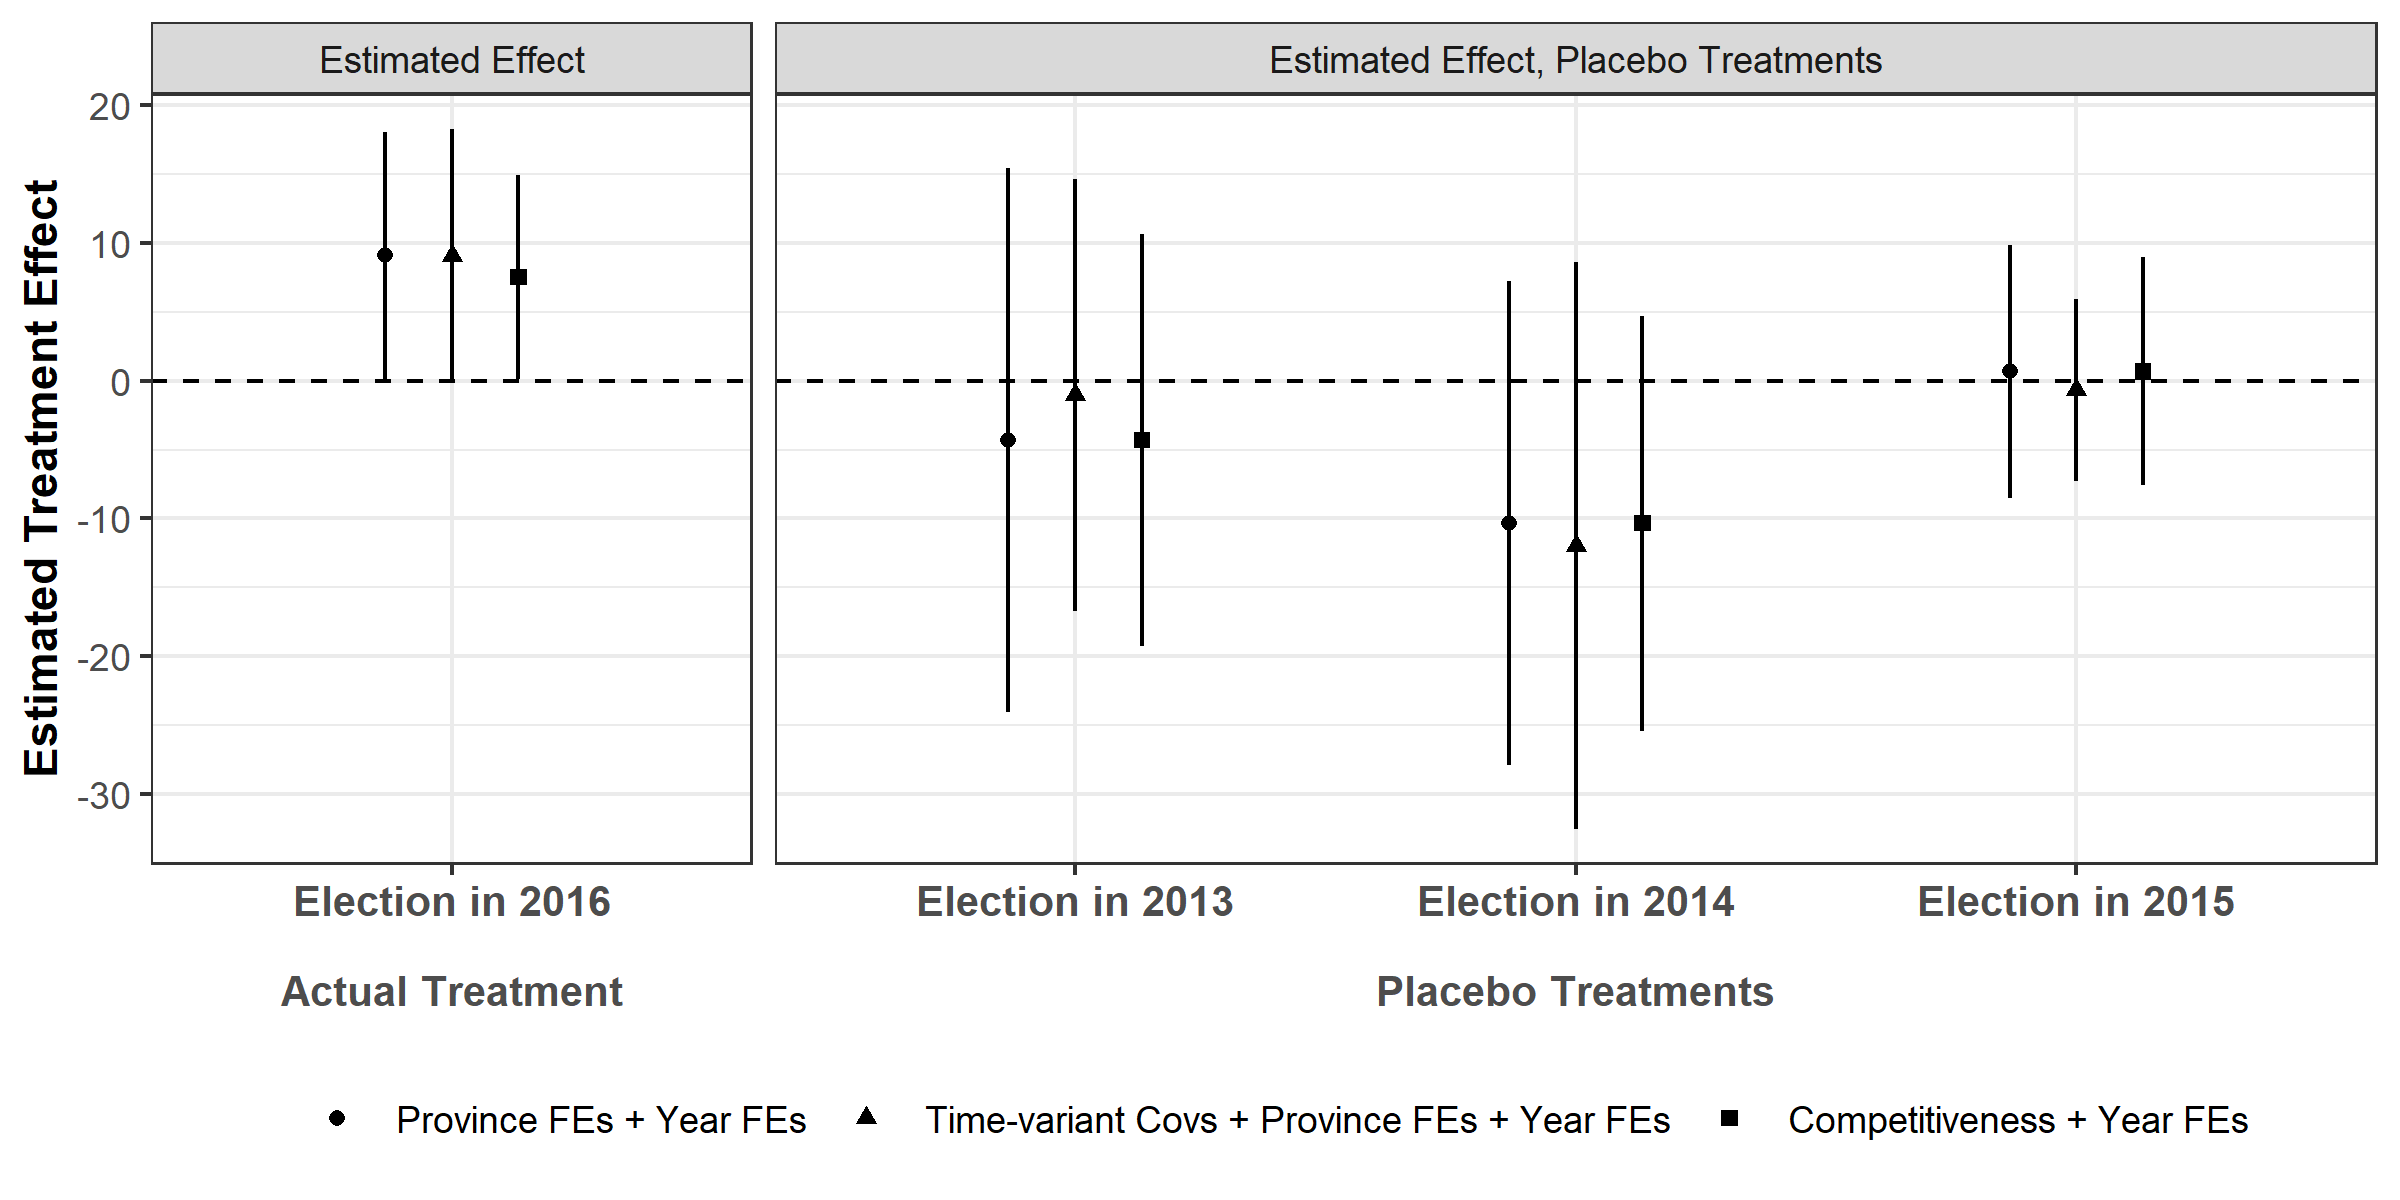
\includegraphics[width=\textwidth]{figure/200422_lfe_placebo.png}
	\captionsetup{singlelinecheck=off}
	\caption[Estimated placebo linear fixed effects treatment effects]{Estimates of instantaneous treatment effects using linear fixed effects models. The error bars show 95\% confidence intervals.}
	\label{fig:lfe_placebo}
\end{figure}

Figure \ref{fig:rdd_placebo} presents the results from the regression discontinuity analysis. Since this analysis uses a randomization procedure that does not rely on large sample asymptotics, its inferences are not subjected to the small sample concerns that may have cast doubt on the previous results. Reassuringly, the results show the treatment effect to be statistically similar to those found in Table \ref{tab:lfe_main}. Specifically, the estimated effect of losing central candidates is estimated to be a 10\% addition to a province's annual change in central transfers. The placebo results suggest that imbalance between treated and untreated provinces are small and close to zero. Similar to Figure \ref{fig:lfe_placebo}, a negative but statistically insignificant difference is detected for the 2014 placebo. 

\begin{figure}[!htbp]
	\centering
	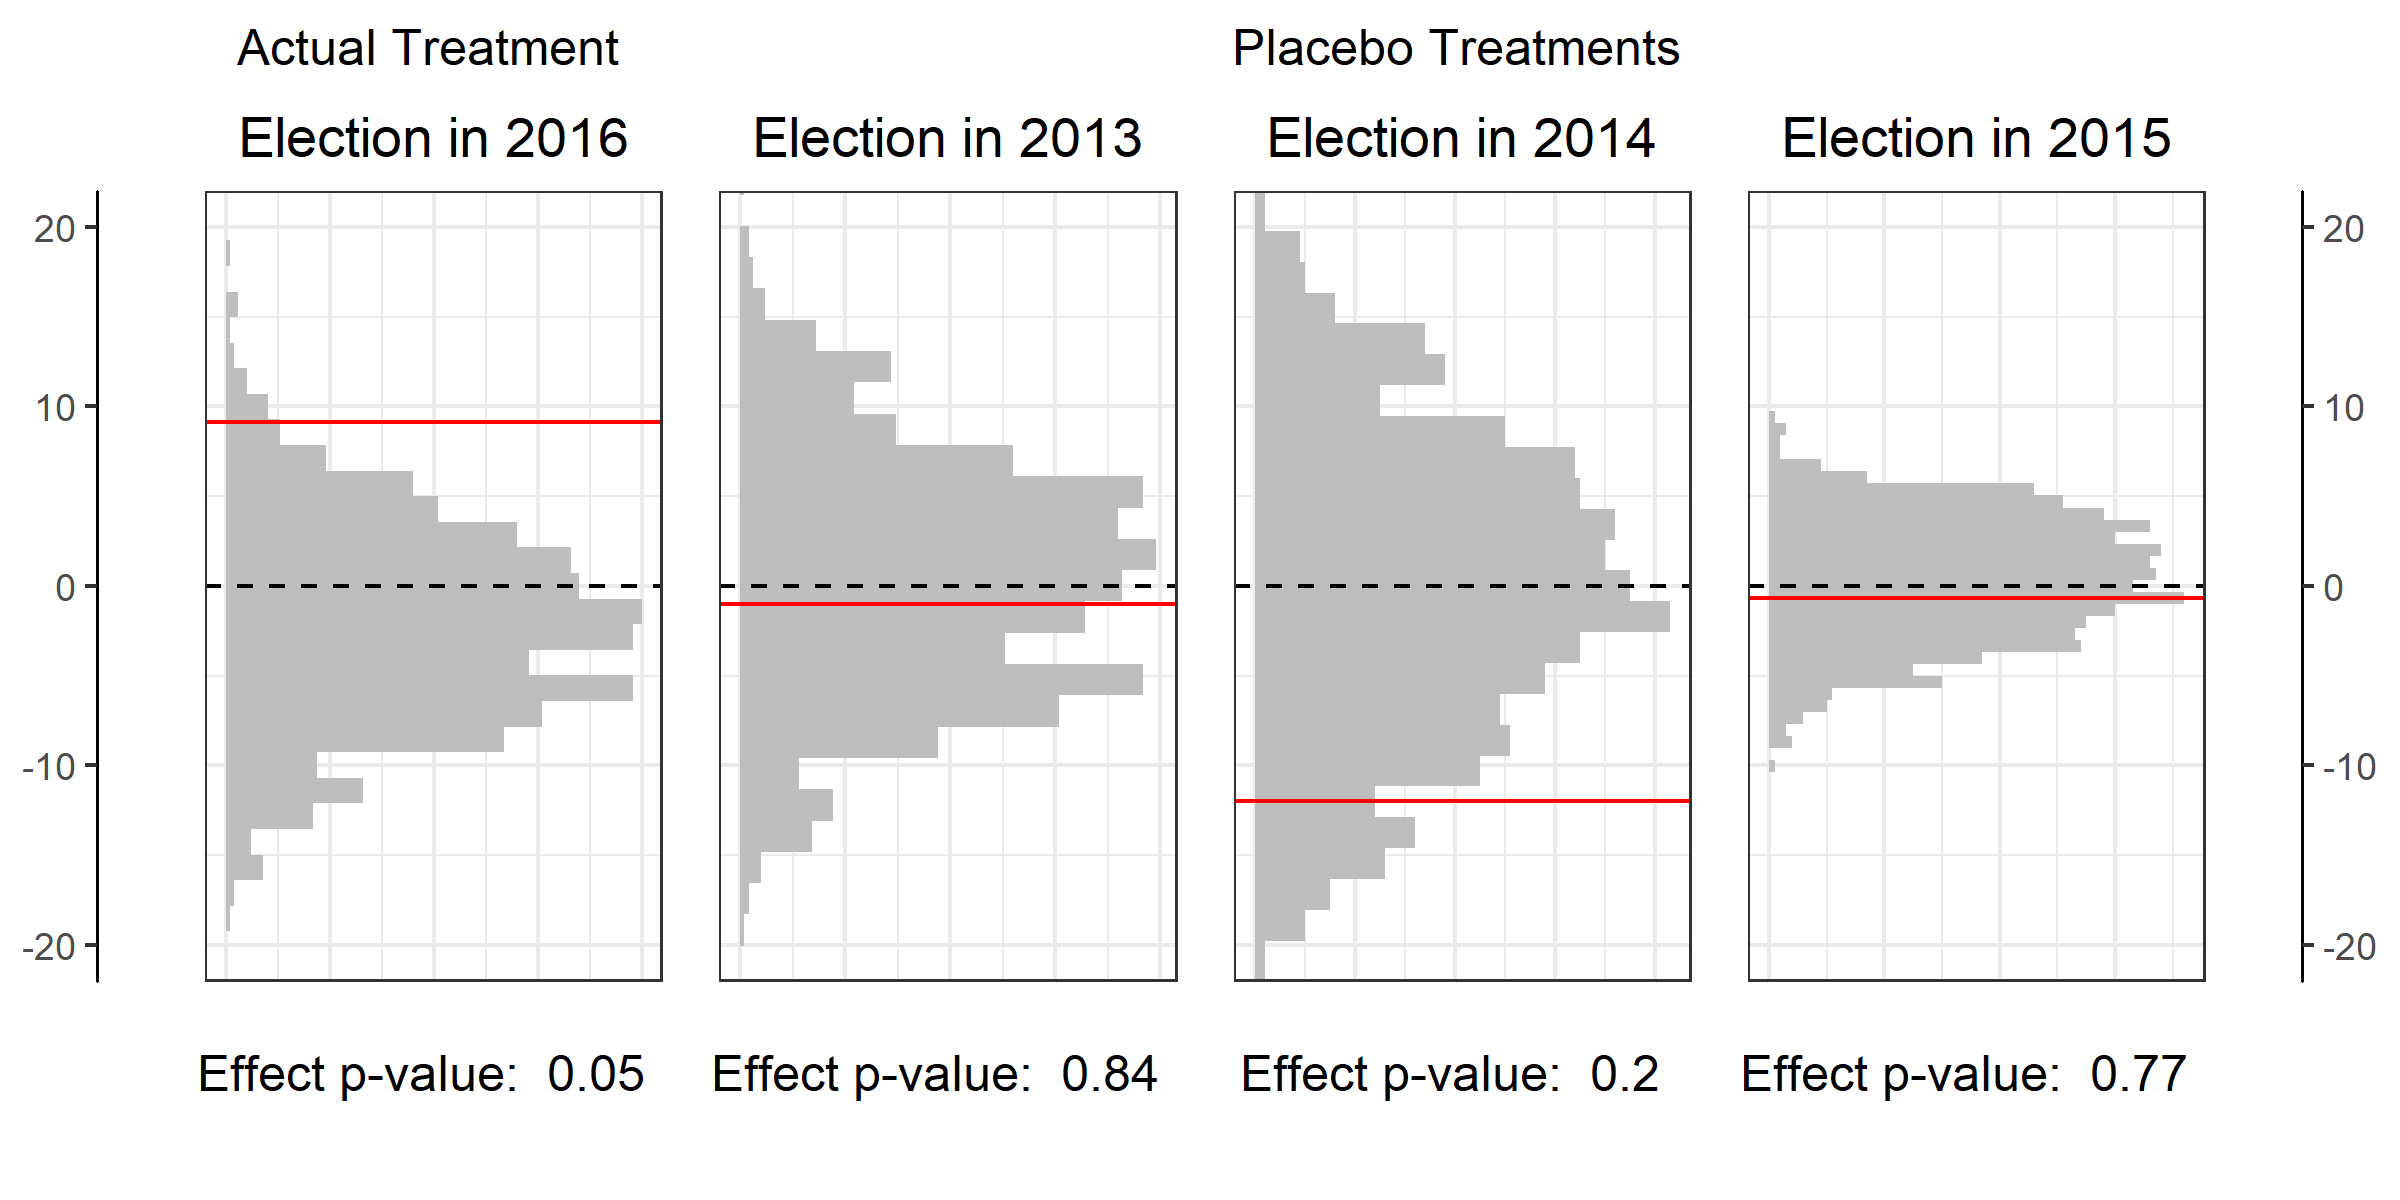
\includegraphics[width=\textwidth]{figure/200422_rdd_results.png}
	\captionsetup{singlelinecheck=off}
	\caption[Estimated RDD treatment effects]{Estimates of instantaneous treatment effects for RDD analyses using the local randomization approach. The red lines show the estimated treatment effects, and the gray bars show their randomization distribution. P-values are presented for the treatment effect estimate.}
	\label{fig:rdd_placebo}
\end{figure}

The absence of statistically significant placebo effects in Table \ref{tab:lfe_main} and Figure \ref{fig:rdd_placebo} suggests only minor threat of dynamic causality. However, to remain as conservative as possible, I conduct an additional analysis using the generalized synthetic control method, which is particularly effective at addressing dynamic causality. The results, shown in Figure \ref{fig:synth_placebo}, confirm not only a significant (at the .1 level) and sustained treatment effect for 2017 and 2018, but also the absence of any difference across treated units and the synthetic control in the years prior to the election. The magnitude of the treatment effect is consistent with previous results.

\begin{figure}[!htbp]
	\centering
	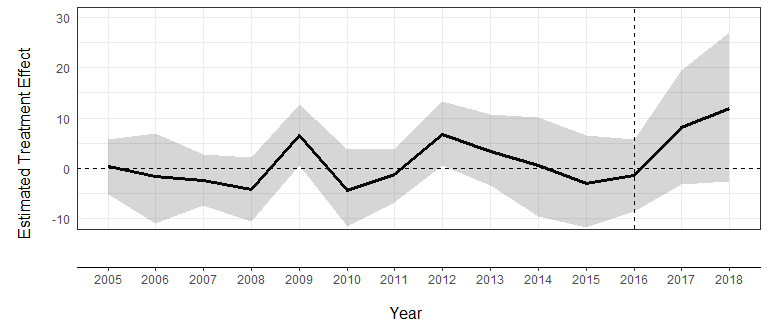
\includegraphics[width=\textwidth]{figure/200422_synth_results.png}
	\captionsetup{singlelinecheck=off}
	\caption[Estimated synthetic control treatment effects]{Estimates of treatment effects using the generalized synthetic control method. The horizontal dashed line marks the election year.}
	\label{fig:synth_placebo}
\end{figure}

Altogether, the three different analyses present a consistent set of findings, according to which the central government in Vietnam increased the amount of central transfers to provinces that suffered defeats of central candidates in the 2016 election. The resulting treatment effect is statistically and substantively significant across all specifications, and have survived sufficient placebo tests. The small sample size, particularly the number of provinces with central candidate defeats, may be a cause for concern, but in Online Appendix \ref{app:small_sample} I show that it does not compromise the finding's validity. Overall, the robust findings lend credibility to the hypothesis that the CPV leadership considered election setbacks as indicators for areas of low regime support, and chose to remedy this problem by increasing central support to these areas.

\section{Additional Evidence}
\label{sec:additional}

\subsection{Responses to Localized Defeats in Previous Elections}

The above conclusion depends on whether the CPV's increases in central transfers are truly  a conscious response to central candidate defeats and part of their efforts to maintain public support across Vietnam's many sub-national units. To confirm this, I show that the empirical patterns observed for the 2016 election are not artifacts of an important time-varying confounder, and that they are likely to hold for previous elections as well.

The time-varying confounding factor in question arises from a revised State Budget Law, which was issued in 2015 and began taking effect in 2017. It has resulted in significant changes to budget allocations among some Vietnamese provinces \citep{BaoViet2016}, which could possibly be mistakenly counted in the treatment effect estimates. In Online Appendix \ref{app:budget_law} (5-6), however, I show that there is no overlap between provinces affected by the 2015 State Budget Law and provinces included in my sample.

Showing that the main results hold for previous elections proves to be no easy task: election data is available for only two of the most recent elections in 2007 and 2011, and even then it is not complete. Specifically, for the 2007 and 2011 elections no vote share data is available for defeated candidates, which prevents any attempt at identifying and separating out central candidates who lost or won narrowly from those who did so with large margins. In Online Appendix \ref{app:previous_elections} (7-17), I argue and demonstrate that failing to identify close defeats lead to unbalanced samples and consequently invalid estimates. However, the best-available analysis using the generalized synthetic control method to reduce dynamic causality for the 2011 sample produces positive and statistically significant estimates of the treatment effect (this method is not appropriate for the 2007 sample). In addition, after calculating all feasible treatment effects by simulating possible values of the unobserved vote shares, I find that the true treatment effects -- which would have been identified had vote shares in 2007 and 2011 been fully observed -- are very likely to be positive. Altogether, these attempts to mitigate the data limitation produce some tentative but still consistent results, according to which the CPV also increased central transfers to provinces with localized defeats in the 2007 and 2011 elections.

\subsection{Effect of Increased Central Transfers}

Another key component of the conclusion is that the CPV increased central transfers to areas it observes weaker regime support specifically to placate the dissatisfied voting public. For this to happen, the increased flow of money should have been spent on public goods that directly benefit citizens. In addition, there should have been no significant re-allocation of expenditure from items that benefit local officials to those that benefit citizens, or else the net increase in central transfers would still mask a direct punishment to provincial leaders. 

I find evidence to verify both propositions by looking at two line items in each province's budget: development spending, which consists mostly of investment on public projects, and administrative spending, which includes from large procurement orders to recurrent expenses such as salaries, travel reimbursements or even office supplies, most of which directly affect the livelihood of provincial bureaucrats. Straightforwardly, an increase in development spending would be evident of placation towards citizens, whereas cuts in administrative spending would suggest punishment towards provincial officials. In Online Appendix \ref{app:mechanisms} (18-19), I show that available data confirms the former, but offers no support for the latter.

\subsection{Alternative Mechanisms for Increased Central Transfers}

An alternative interpretation of the empirical results is that the increase in downward flow of money, even if being channeled towards public goods, may not reflect a top-down decision to buy off the public, but was instead the result of bottom-up demand. From this perspective, localized defeats led to increased central transfers not because they sent a signal from the provinces to Hanoi, but because each defeated central candidate left a seat for local elites to fill, strengthening the province's representation and bargaining power in the legislature.

In Online Appendix \ref{app:alt_mech} (p. 20), I rule out this alternative explanation after looking at the province of Can Tho, where central candidate lost because they and other candidates failed to clear the 50 percent threshold. This province ended up with an unfilled seat and no increased representation. However, its individual treatment effect, estimable thanks to the generalized synthetic control, is still positive and large in size, ruling out negotiation and bargaining through representation as the driver behind central transfers increases.

\section{Discussion and Conclusion}

\subsection{Insight from the Vietnam case}

The thriving literature on authoritarian institutions in general and authoritarian elections in particular has identified a number of governance goals that these elections can achieve, many of which center around their ability to provide information that authoritarian regimes cannot access easily. Left unconsidered by this literature, however, is the reality that each authoritarian regime can only seek and receive a limited amount of information from elections, no matter how many different signals they can emit. As a result, rational autocrats are expected to focus each election towards a limited number of prioritized information goals.

In this paper, I demonstrate how post-election responses to surprising and thus informative localized defeats can reveal which specific information autocrats seek from their elections. Applying this logic to Vietnam, this paper finds that Vietnam's leaders increased central transfers to provinces with such defeats in the 2016 legislative election. This response suggests that the regime has used election to learn about the geographic distribution of its popularity, and thus saw the defeats as indicators for areas with low support in need of financial placation. It also rejects the possibility that Hanoi used elections to evaluate the ability of provincial officials to manage elections, because if so it would have seen the defeats as revealing incompetent or disloyal officials deserving of punishment. Increasing central transfers would accomplish only the opposite. An array of additional evidence proves consistent with this conclusion.

Precisely because its empirical evidence draws from the case of Vietnam, this paper's findings may contribute significantly to the understanding of authoritarian resilience in other areas of the world. Specifically, if even this strong, highly institutionalized, single-party regime, with all the power needed to consistently command near-perfect election results, still cannot satisfy all its information needs by holding authoritarian elections, then perhaps there really is an upper limit to how much assistance elections and other authoritarian institutions could provide for the dictators of the world. In addition, the Vietnamese regime's decision to prioritize signals about its popularity suggests that autocrats listen and do respond to public dissatisfaction. This echoes other findings in the literature that even formal authoritarian institutions may offer pathways to accountability \citep[e.g.][]{Miller2015}, but calls into questions existing claims that autocrats pay more attention to governing their own subordinates than to keeping citizens content \citep[e.g.][]{Svolik2012}.

\subsection{Generalizability of empirical framework}

This paper also contributes an empirical framework against which informational theories of authoritarian elections could be tested. This test is needed when there are multiple plausible but contradictory motivations for autocrats to hold elections, which means that at least some theories about these motivations must be at odds with reality. The paper applies this test to the Vietnam case to adjudicate between a theory that suggests autocrats hold elections to better measure public support for the national regime, and one that claims they do so to learn about local agents' quality. This specific theoretical tension arises because elections in Vietnam can be informative on both types of information, making both motivations plausible. The same situation applies to many other cases of authoritarian regimes. Given that almost all authoritarian elections can be informative of agent performance, as long as autocrats delegate electoral manipulation to their subordinates, a large number of these elections may simultaneously be informative of public approval for the regime. This is clearly the case in presidential systems, where incumbent executives personify their entire regimes on the ballot. Yet it also applies to a large number of other parliamentarian autocracies where central and local candidates are not institutionally separated, because relevant actors may still have information to determine each candidate's alignment if they need to.\footnote{In China, for example, voters rely on the candidates' records to identify ``governance types'' who are closer to the regime \citep{Manion2014}. In Uganda, even among candidates put forward by the ruling NRM party, those selected through the party primaries are well-known to be closer to the party leadership than those who entered as individuals \citep{TK}.} 

Less common, however, are situations in which elections may provide \textit{only one} of these two types of information, a condition needed for the test to uniquely identify one single purpose of authoritarian elections. In the case of Vietnam, this condition is met thanks to the CPV's careful pre-election engineering. In many other electoral autocracies, closed-list PR, such as in TK-examples \citep{TK}, or heavily restricted space for campaigning, such as in Singapore \citep{TK}, may achieve the same. All of these are examples of \textit{selective manipulation}, the strategy by which an authoritarian regime uses manipulation tactics to shut down some sources of influence on election results but still tolerate some others. While it is beyond the scope of this paper to identify the complete universe of cases for which its empirical test would apply, it argues that evidence of selective manipulation provides a good indicator.

More generally, beyond this particular empirical test, the general framework demonstrated in this paper could be useful for other cases, to adjudicate between different sets of motivations for authoritarian elections. As the starting point, researchers need to identify an authoritarian regime's informational needs and detect whether selective manipulation is at work to make elections plausibly satisfy these needs. Then, as long as they can extend existing theories to establish logical hypotheses linking each informational need with an appropriate response to incoming information from elections and identify whether any pair of hypotheses imply contradictory responses, observing the regime's reactions to surprising localized upsets can help rule out theories that do not hold true for the given case. 

Given this framework, the specifics of the test can and should be flexibly adapted to each individual case. For example, different country cases may require different operationalization of electoral upsets, as long as they are sufficiently surprising and yet not existentially threatening. Thus, just as scholars of one-party systems focus on rare localized defeats, students of more competitive electoral autocracies may prioritize big vote swings or low incumbent vote shares. Similarly, researchers are not restricted to studying post-election budget allocations, but should use their case knowledge to identify the kind of post-election response that would offer the most inferential leverage for each country. Both these steps are easiest when studying authoritarian regimes with limited policy discretion, which describes most highly-institutionalized, single- or dominant-party states such as Vietnam, China, or Singapore, as well as a broad range of other hybrid regimes whose leaders are constrained by weak state capacity rather than institutionalization, but the general framework is not exclusively restricted to these cases. 

Ultimately, what this paper offers is a rigorous case-level test of potentially competing theories of authoritarian elections. It leverages particular institutional features in one authoritarian regime, and demonstrates the limits of at least one existing theory when applied to that regime. This approach may help bridge existing theory-building using country cases \citep[e.g.][]{Magaloni2006, Blaydes2010} with theory-testing using cross-national studies \citep[e.g.][]{Miller2015}, which may omit significant heterogeneity across different regimes.

%It is important not to overstate its scope conditions, however. The test demonstrated in this paper works because the two most plausible theories happen to predict two post-election responses with opposite observable implications in Vietnam; this is not necessarily the case elsewhere.  For example, as \citet{Magaloni2006} and \citet{Blaydes2010} find in their studies of Mexico and Egypt, the ruling parties respond to information about areas of relatively low popularity by cutting their government funding. In these cases, this ``punishment regime'' serves two function: weaken opposition party-building and deter voters from supporting the opposition. In Vietnam, neither is necessary. First, there is no organized opposition to be weakened. Second, without an organized opposition, localized defeats reflect only diffused dissatisfaction towards the CPV and not a mobilized movement gaining in momentum. For the CPV, reducing this dissatisfaction is more important than bullying voters into voting the right way -- it already has other instruments which could achieve this goal but which it has chosen not to use. In addition, even in areas with localized defeats the absolute level of support for the regime is still high, which means that cutting transfers would hurt regime supporters more than it punishes dissidents. 

%Although cross-national evidence by \citet{Miller2015} indicates a prevalence of placation strategies, cases like Mexico and Egypt are not rare: in many hybrid regimes, the possibility of dissenting citizens being mobilized is enough for punishment regimes to become necessary. Furthermore, in many other contexts, the plausible informational goals that outside observers need to discern from may neither be related to the regime's popularity nor its agents' quality. Under these circumstances, this specific empirical test will not apply. 

%The general framework of the test, however, remains valid, as long as researchers can extend existing theories to identify logical plausible hypotheses about appropriate responses to incoming information from elections, and then identify whether any pair of responses are practically contradictory given the country case's context. Thus, it would work best in situations when authoritarian regimes have limited policy discretion, which describes most highly-institutionalized, single- or dominant-party states such as Vietnam, China, or Singapore, but also a broad range of other hybrid regimes whose leaders are constrained by weak state capacity rather than institutionalization.

%\singlespacing
\inputencoding{utf8}
\printbibliography[heading=bibintoc]

\end{document}